\documentclass[beamer,11pt,aspectratio=169]{beamer}

\usepackage{pgf}
\usepackage{tikz}
\usepackage{pgfplots}
\usepackage{xcolor}
\usepackage[finnish]{babel}
\usepackage[utf8]{inputenc}
\usepackage{textcomp}
\usepackage[T1]{fontenc}
\usepackage{microtype}
\usepackage{textgreek}
\usepackage{multirow}
\usepackage{booktabs}
\usepackage{bm}
\usepackage{graphicx}
\usepackage{amsmath}
\usepackage{gensymb}
\usepackage{booktabs}
\usepackage{tabularx}
\usepackage{tikz-feynman}
\usepackage{animate}
\usepackage{xmpmulti}
\usepackage{hyperref}
\usepackage{luacode}
\usepackage{unicode-math}
\usepackage{pdfrender}
\usepackage{pbox}

%\usepackage[short]{journalnames}
\usepackage{scpcolors}

%  BIBLIOGRAPHY
\usepackage[backend = biber,
           language = english,
            citestyle = authoryear,
            bibstyle = authortitle,
            sorting = nyt,
            giveninits = true,
            minbibnames = 1,
            mincitenames = 1,
            maxbibnames = 2,
            maxcitenames = 2,
            hyperref = true,
            arxiv = abs,
            uniquename = false]{biblatex}

\AtEveryBibitem{\clearfield{title}\clearfield{doi}\clearfield{issn}\clearfield{url}\clearfield{primaryClass}}

\addbibresource{zebra_seminar.bib}

\renewcommand*{\bibnamedash}{\rule[0.48ex]{3em}{0.14ex}\space}
\renewcommand*{\bibnamedelimi}{\hspace{0.125em}}
\renewcommand*{\mkbibacro}[1]{#1}
\renewbibmacro{in:}{}

\newcommand{\journaltitlecolor}{grey1}

\pgfplotsset{compat=newest}
\usetikzlibrary{decorations.pathmorphing}
\usetikzlibrary{decorations.text}
\usetikzlibrary{fadings}
\usetikzlibrary{pgfplots.groupplots}
\usetikzlibrary{backgrounds}
\usetikzlibrary{external}
\usepgflibrary{shadings}

\usepgfplotslibrary{colorbrewer}
\usepgfplotslibrary{fillbetween}
\usepgfplotslibrary{extracolormaps}

%\pgfplotsset{legend image code/.code={\draw[#1](0,-0.0125)rectangle(0.06,0.0225);}}

%  vector differential operators
\newcommand{\Nabla}{\bm{\nabla}}
\newcommand{\Div}{\Nabla\cdot}
\newcommand{\Curl}{\Nabla\times}

%  derivatives
\newcommand{\tder}[2]{d#1/d#2}
\newcommand{\der}[2]{\frac{d#1}{d#2}}
\newcommand{\dder}[2]{\frac{d^2#1}{d#2^2}}
\newcommand{\dern}[3]{\frac{d^{#3}#1}{d#2^{#3}}}
\newcommand{\ddder}[3]{\frac{d^2#1}{d#2d#3}}
\newcommand{\inder}[2]{\frac{\mathfrak{d}#1}{\mathfrak{d}#2}}

%  partial derivatives
\newcommand{\pder}[2]{\frac{\partial#1}{\partial#2}}
\newcommand{\pdder}[2]{\frac{\partial^2#1}{\partial#2^2}}
\newcommand{\ppder}[3]{\frac{\partial^2#1}{\partial#2\partial#3}}
\newcommand{\pdern}[3]{\frac{\partial^{#3}#1}{\partial#2^{#3}}}
\newcommand{\tpder}[2]{\partial#1/\partial#2}

%  miscellaneous
\newcommand{\unitv}[1]{\hat{#1}}
\newcommand{\difd}{\,d}
\newcommand{\mean}[1]{\left\langle#1\right\rangle}
\newcommand{\smean}[1]{\langle#1\rangle}
\newcommand{\vblank}{\vspace{1pc}}
\newcommand{\imp}[1]{\textsf{#1}}
\newcommand{\needcite}{\textcolor{darkred}{[citation needed]}}
\newcommand{\cited}[1]{\textcolor{darkred}{[#1]}}
\newcommand{\lssc}[1]{\textls[70]{\textsc{#1}}}
\newcommand{\reffig}[1]{Fig. \ref{#1}}
\newcommand{\transp}{\mathsf{T}}
\newcommand{\mand}{\quad\text{and}\quad}
\newcommand{\bra}[1]{\left\langle#1\right|}
\newcommand{\ket}[1]{\left|#1\right\rangle}
\newcommand{\braket}[2]{\left\langle#1\middle|#2\right\rangle}
\newcommand{\brakett}[3]{\left\langle#1\middle|#2\middle|#3\right\rangle}
\newcommand{\frgn}[1]{\textit{#1}}
\newcommand{\faml}[1]{#1}
\newcommand{\name}[1]{\textit{#1}}
\newcommand{\normal}{\trianglelefteq}
\newcommand{\zmod}[1]{\mathbb{Z}/{#1}\mathbb{Z}}
\newcommand{\bsf}[1]{\bm{\mathsf{#1}}}
\newcommand{\cat}[1]{\mathsf{#1}}
\newcommand{\secnote}[1]{\textit{\color{darkreddish} #1}\par\noindent}
\newcommand{\important}[1]{{\sffamily #1}}
\newcommand{\nothing}[1]{}

%  spacing
\newcommand{\nen}{\hspace{-5pt}}
\newcommand{\nquad}{\hspace{-10pt}}
\newcommand{\nqquad}{\hspace{-20pt}}

\DeclareMathOperator{\im}{im}
\DeclareMathOperator{\diag}{diag}
\DeclareMathOperator{\id}{id}
\DeclareMathOperator{\Aut}{Aut}
\DeclareMathOperator{\lcm}{lcm}
\DeclareMathOperator{\Inn}{Inn}
\DeclareMathOperator{\chara}{char}
\DeclareMathOperator{\sgn}{sgn}
\DeclareMathOperator{\rad}{rad}
\DeclareMathOperator{\Hom}{Hom}
\DeclareMathOperator{\End}{End}
\DeclareMathOperator{\Sym}{Sym}
\DeclareMathOperator{\Ant}{Ant}
\DeclareMathOperator{\Int}{int}
\DeclareMathOperator{\supp}{supp}
\DeclareMathOperator{\rank}{rank}
\DeclareMathOperator{\Lie}{Lie}
\DeclareMathOperator{\tr}{tr}
\DeclareMathOperator{\tdet}{det}
\DeclareMathOperator{\Li}{Li}
\DeclareMathOperator{\Br}{Br}
\DeclareMathOperator{\erf}{erf}

\definecolor{grey}{gray}{0.8}
\definecolor{grey1}{gray}{0.05}
\definecolor{grey2}{gray}{0.8}
\definecolor{grey3}{gray}{0.5}
\definecolor{lightred}{RGB}{90, 50, 50}
\definecolor{darkerred}{RGB}{90, 10, 10}
\definecolor{darkred}{rgb}{0.3,0,0}
\definecolor{somered}{rgb}{0.7,0,0}
\definecolor{grape}{RGB}{76,40,130}
\definecolor{frenchviolet}{Hsb}{279,0.97,0.4}
\definecolor{mardigras}{Hsb}{301,1,0.2}
\definecolor{indigo}{Hsb}{255,1,0.4}
\definecolor{mediumblue}{Hsb}{240,0.2,0.8}
\definecolor{indigobright}{Hsb}{255,0.8,0.65}
\definecolor{turqoise}{RGB}{91, 146, 121}

\definecolor{detector}{Hsb}{111,0.6,0.65}
\definecolor{fieldtheory}{Hsb}{348,0.9,0.75}
\definecolor{halo}{Hsb}{255,0.65,0.75}



\definecolor{proton-red}{RGB}{212, 65, 65}

\newcommand{\shadecolor}{indigo}
\newcommand{\defaulttextcolor}{white!70!black}
\newcommand{\defaultbgcolor}{grey1}

\setmainfont{Noto Sans}[
    BoldFont = Noto Sans Bold,
    ItalicFont = Noto Sans Italic,
    BoldItalicFont = Noto Sans Bold Italic
]
\setsansfont{Noto Sans}[
    Ligatures = {
        NoCommon, NoDiscretionary, NoHistoric, NoRequired, NoContextual
    }
]
\setmonofont{Noto Mono}
\setmathfont{Noto Sans Math}

% Semibold fonts
\newfontface\sbstyle{Noto Sans Semibold}

% Some special styles
%\newcommand{\titlestyle}{\sbstyle}
\newcommand{\annotatestyle}{\sbstyle}
%\newcommand{\headstyle}{\sbstyle}
%\newcommand{\subheadstyle}{\sbstyle}
%\newcommand{\subsubheadstyle}{\sbstyle}

% Additional commands for typesetting semibold (sb) and uppercase (uc) text in
% serif and sans serif (sf) style
\newcommand{\textsb}[1]{{\sbstyle #1}}
\newcommand{\textuc}[1]{\textls[70]{#1}}

%\SetTblrStyle{remark-tag}{font=\itshape}
%\SetTblrStyle{remark-sep}{font=\itshape}
%\SetTblrStyle{caption-tag}{font=\bfseries}
%\SetTblrStyle{caption}{halign=l}

% Redefine vector command to use bold italics
%\renewcommand{\vec}[1]{\symbfit{#1}}

% Special typesetting for annotating plots
\newcommand{\plotlineannotation}[1]{{\tiny\annotatestyle #1}}

\renewcommand*{\emph}[1]{\textit{#1}}

\setbeamersize{text margin left=5mm,text margin right=5mm} 

\setbeamertemplate{footline}[text line]{%
  \parbox{\linewidth}{\insertshortauthor\vspace{-5pt}\hfill\insertframenumber\vspace{5pt}}}
\setbeamertemplate{navigation symbols}{}

\setbeamercolor{palette primary}{fg=\defaulttextcolor}
\setbeamercolor{palette secondary}{fg=\defaulttextcolor}
\setbeamercolor{palette tertiary}{fg=\defaulttextcolor}
\setbeamercolor{palette quarternary}{fg=\defaulttextcolor}
\setbeamercolor{palette sidebar primary}{fg=\defaulttextcolor}
\setbeamercolor{palette sidebar secondary}{fg=\defaulttextcolor}
\setbeamercolor{palette sidebar tertiary}{fg=\defaulttextcolor}
\setbeamercolor{palette sidebar quarternary}{fg=\defaulttextcolor}
\setbeamercolor{palette primary}{fg=\defaulttextcolor}
\setbeamercolor{palette primary}{fg=\defaulttextcolor}
\setbeamercolor{palette primary}{fg=\defaulttextcolor}

\setbeamercolor{normal text}{bg=\defaultbgcolor,fg=\defaulttextcolor}
\setbeamercolor{titlelike}{fg=\defaulttextcolor}
\setbeamercolor{alerted text}{fg=\defaulttextcolor}
\setbeamercolor{example text}{fg=\defaulttextcolor}
\setbeamercolor{structure}{fg=\defaultextcolor}
%\setbeamercolor{separation line}{fg=grey1,bg=grey1}
%\setbeamercolor{fine separation line}{fg=grey1,bg=grey1}

\setbeamercolor{title page}{fg=\defaulttextcolor}
\setbeamercolor{title}{fg=\defaulttextcolor}
\setbeamercolor{subtitle}{fg=\defaulttextcolor}
\setbeamercolor{author}{fg=\defaulttextcolor}
\setbeamercolor{institute}{fg=\defaulttextcolor}
\setbeamercolor{date}{fg=\defaulttextcolor}

\setbeamercolor{part page}{fg=\defaulttextcolor}
\setbeamercolor{section page}{fg=\defaulttextcolor}
\setbeamercolor{subsection page}{fg=\defaulttextcolor}

\setbeamercolor{section in toc}{fg=\defaulttextcolor}
\setbeamercolor{subsection in toc}{fg=\defaulttextcolor}
\setbeamercolor{subsubsection in toc}{fg=\defaulttextcolor}
\setbeamercolor{section in toc shaded}{fg=\defaulttextcolor}
\setbeamercolor{subsection in toc shaded}{fg=\defaulttextcolor}
\setbeamercolor{subsubsection in toc shaded}{fg=\defaulttextcolor}
\setbeamercolor{section number projected}{fg=\defaulttextcolor}

\setbeamercolor{bibliography entry title}{fg=\defaulttextcolor}
\setbeamercolor{bibliography entry location}{fg=\defaulttextcolor}
\setbeamercolor{bibliography entry author}{fg=\defaulttextcolor}
\setbeamercolor*{bibliography entry note}{fg=\defaulttextcolor}
\setbeamercolor{bibliography item}{fg=\defaulttextcolor}

\setbeamercolor{note page}{fg=\defaulttextcolor}

\setbeamercolor{background canvas}{fg=\defaultbgcolor}
\setbeamercolor{background}{bg=\defaultbgcolor}

\setbeamercolor{headline}{fg=\defaulttextcolor}
\setbeamercolor{footline}{fg=\defaulttextcolor}
\setbeamercolor{page number in head}{fg=\defaulttextcolor}
\setbeamercolor{page number in foot}{fg=\defaulttextcolor}

\setbeamercolor{button}{fg=\defaulttextcolor}

\setbeamercolor{structure}{fg=\defaulttextcolor}

%\setbeamercolor{}

\setbeamertemplate{itemize item}{\color{\defaulttextcolor}\textbullet}
\setbeamertemplate{itemize subitem}{\color{\defaulttextcolor}\textbullet}
\setbeamertemplate{itemize subsubitem}{\color{\defaulttextcolor}\textbullet}
\setbeamertemplate{enumerate item}{\color{\defaulttextcolor}\arabic{enumi})}
\setbeamertemplate{bibliography item}

\renewcommand*{\bibfont}{\scriptsize}

\newcommand{\defaultaccentcolor}{turqoise}
\hypersetup{
    colorlinks=true,
    citecolor=\defaulttextcolor,
    linkcolor=\defaultaccentcolor,
    urlcolor=\defaultaccentcolor
}

\newcommand{\scale}{0.7}
\tikzset{
    box/.pic={
        \fill[fill opacity=1.0](0,0)--(0.866,0.5)--(0,1)--(-0.866,0.5)--cycle;
        \fill[fill opacity=0.0](0,0)--(-0.866,0.5)--(-0.866,-0.5)--(0,-1)--cycle;
        \fill[fill opacity=0.5](0,0)--(0,-1)--(0.866,-0.5)--(0.866,0.5)--cycle;
    }
}

\tikzset{
    hexagon/.pic={
        \fill[fill opacity=1.0](0.866,0.5)--(0,1)--(-0.866,0.5)--(-0.866,-0.5)--(0,-1)--(0.866,-0.5)--cycle;
        \fill[fill opacity=0.7](0,0)--(-0.866,0.5)--(-0.866,-0.5)--(0,-1)--cycle;
        \fill[fill opacity=0.4](0,0)--(0,-1)--(0.866,-0.5)--(0.866,0.5)--cycle;
    }
}

\tikzset{
    cross/.pic={
        \draw [thick] (0.4,0.4)--(0.1,0.1);
        \draw [thick] (-0.4,0.4)--(-0.1,0.1);
        \draw [thick] (0.4,-0.4)--(0.1,-0.1);
        \draw [thick] (-0.4,-0.4)--(-0.1,-0.1);
    }
}

\begin{luacode*}

function mix(x, y, a)
    return x*(1 - a) + y*a
end

function hash(n)
    return math.abs(math.fmod(math.sin(n)*1.0e+4, 1.0))
end

function noise(x)
    i = math.floor(x)
    f = math.fmod(x, 1.0)
    u = f*f*(3.0 - 2.0*f)
    return mix(hash(i), hash(i + 1.0), u)
end

function scaled_noise(x)
    return 1 - 2.0*noise(x)
end

function length(x, y)
    return math.sqrt(x*x + y*y)
end

function density(xpos, ypos)
	t = 1.5
    k = 1.4
    w = 2.0
    c = w/k
    center_x = 1.0
    center_y = 0.5
    x = xpos - center_x
    y = ypos - center_y
    tp = t - length(x, y)/c
    ppx = scaled_noise(0.48*tp)
    ppy = scaled_noise(0.56*tp + 1.0)
    x = xpos - ppx
    y = ypos - ppy
    return math.pow(noise(k*length(x, y) - w*t), 1)
end

function density2(xpos, ypos)
    center_x = 0.6
    center_y = 0.5
    x = xpos - center_x
    y = ypos - center_y
    r = math.sqrt(x*x + 0.5*y*y)
    res = math.sin(2.0*r)
    if math.random() < 0.5 then
        return math.random()*math.pow(res, 10)
    else
	    return math.pow(res, 10)
    end
end

function print_opacity(i, j, N, M)
    dens = density2(tonumber(i)/tonumber(N), tonumber(j)/tonumber(M))
	 tex.print(tostring(dens))
end

function test(x)
	y = x:gsub("pt","")
	return tonumber(y)
end

function triangle_base(pageheight, N)
    tex.print(string.format("%f",test(pageheight)*0.03528/tonumber(N)))
end

function horizontal(pagewidth, pageheight, N)
    tex.print(string.format("%d",math.ceil((0.5/0.866)*tonumber(N)*test(pagewidth)/test(pageheight))))
end

function randbin()
	r = math.random()
	res = 0
	if r > 0.5 then
	    res = 1
   end
   tex.print(string.format("%d",res))
end

function increment(n)
    tex.print(string.format("%d",tonumber(n) + 1))
end

function lattice_pos(is, js, scale)
    i = tonumber(is)
    j = tonumber(js)
    xpos = i*scale
    ypos = j*scale
    if (i == 2 and j == 2) then
        xpos = xpos + 0.15
        ypos = ypos - 0.1
    end
    tex.print(string.format("(%f,%f)", xpos, ypos))
end

function lattice_defects(is, js, scale)
    i = tonumber(is)
    j = tonumber(js)
    xpos = i*scale
    ypos = j*scale
    if (i == 1 and j == 3) then
        xpos = 1.05
        ypos = 0.35
    end
    tex.print(string.format("(%f,%f)", xpos, ypos))
end

function print_if(opacity)
	if opacity > 0.02 then
		tex.print("\\pic[scale=\\scale,color=\\defaultaccentcolor!50!grey1,opacity=\\opacity]at($(current page.north east)-\\scale*1.0*(\\i,0)-\\scale*1.0*(0,\\j)$){cross};")
	end
end
\end{luacode*}

\newcommand{\horizontal}{25}
\newcommand{\vertical}{14}
\newcommand{\atomcolor}{black!80!white}
\newcommand{\atomsize}{1.2mm}

\usebackgroundtemplate{%
    \hspace*{-14.01mm}
    \vspace*{-14.01mm}
    \begin{tikzpicture}[overlay,remember picture]
        \fill[grey1](current page.north west)rectangle(current page.south east);
        \nothing{
            \luadirect{math.randomseed(\insertframenumber)}
            \foreach \j in {0,1,2,...,\vertical}
            \foreach \i in {0,1,2,...,\horizontal}{
                \pgfmathsetmacro{\opacity}{
                        \luadirect{
                            print_opacity(\luastring{\i}, \luastring{\j}, \luastring{\horizontal}, \luastring{\vertical})
                        }
                    }
                    \luadirect{print_if(\opacity)}
            }
            \fill[blue](1.272,0)circle[radius=0.02];
            \fill[blue](17.272,0)circle[radius=0.02];
        }
    \end{tikzpicture}
}

\title{Pimeä aine uuden sukupolven ilmaisimissa}
\author{Sebastian Sassi}
\institute{Helsingin Yliopisto}
\date{6.3.2025}

%\tikzexternalize
%\tikzset{external/up to date check={md5}}

\pgfplotsset{colormap={accentmap}{color=(\atomcolor) color=(\defaultaccentcolor)}}


\pgfplotsset{cycle list/Set2-8}

\newcommand{\darken}[1]{\alt{{\color{\defaulttextcolor!70!black}#1}}{#1}}

% some useful pgf plots keys for working with beamer
\tikzset{
    invisible/.style = {opacity = 0, text opacity = 0},
    visible on/.style = {alt = {#1{}{invisible}}},
    alt/.code args = {<#1>#2#3}{%
      \alt<#1>{\pgfkeysalso{#2}}{\pgfkeysalso{#3}} % \pgfkeysalso doesn't change the path
    },
    shade color on/.code args = {<#1>#2!#3}{
        \alt<#1>{\pgfkeysalso{color=#2!#3!black}}{\pgfkeysalso{color=#2}}
    },
    tint color on/.code args = {<#1>#2!#3}{
        \alt<#1>{\pgfkeysalso{color=#2!#3!white}}{\pgfkeysalso{color=#2}}
    }
}

\newcommand{\bubblestyle}{dashdotted}
\newcommand{\liquidnoblestyle}{solid}
\newcommand{\semiconductorstyle}{dashed}
\newcommand{\scintcrystalstyle}{densely dotted}

\newcommand{\naifillcolor}{scp-red-light-1}

\newcommand{\naicolor}{scp-red-dark-1}
\newcommand{\cawocolor}{scp-purple-dark-1}
\newcommand{\cfcolor}{scp-green-dark-1}
\newcommand{\xenoncolor}{scp-orange-dark-1}
\newcommand{\argoncolor}{scp-brown-dark-1}
\newcommand{\gecolor}{scp-blue-dark-1}
\newcommand{\sicolor}{scp-grey-dark-1}

\newcommand{\wccolor}{scp-orange-dark-1}
\newcommand{\diamondcolor}{scp-green-dark-1}
\newcommand{\siccolor}{scp-purple-dark-1}
\newcommand{\sapphirecolor}{scp-red-dark-1}
\newcommand{\wcolor}{scp-brown-dark-1}

\newcommand{\nufogcolor}{scp-grey-dark-4}

\newcommand{\ppcnocolor}{scp-blue-dark-1}
\newcommand{\lineneutrinocolor}{scp-orange-dark-1}
\newcommand{\hepbcolor}{scp-grey-dark-1}
\newcommand{\atmocolor}{scp-purple-dark-1}
\newcommand{\dsnbreactorcolor}{scp-grey-light-2}

\newcommand{\primarylinecolor}{scp-blue-dark-1}
\newcommand{\secondarylinecolor}{scp-orange-dark-1}

\newcommand{\infernoaxiscolor}{scp-grey-light-3}

\newcommand{\darkmarkcolor}{scp-grey-dark-4}

\newcommand{\plotbgcolor}{scp-grey-light-2!50!white}
\newcommand{\plotfgcolor}{white}

\newcommand{\distellipselinecolor}{scp-green-dark-2}

% pgf plots styles
\pgfplotsset{
    /pgfplots/xlabel near ticks/.style = {
        /pgfplots/every axis x label/.style = {
            at = {(ticklabel cs:0.5)},
            anchor = near ticklabel,
            font = \scriptsize
        }
    },
    every tick/.append style = {color = \defaulttextcolor},
    every axis/.append style = {
        axis line style = {very thick},
        color = \defaulttextcolor,
        xlabel style = {font = \scriptsize},
        ylabel style = {font = \scriptsize},
        tick label style = {font = \tiny},
        title style = {font = \scriptsize}
    },
    every colorbar horizontal post/.append style = {
        xtick style = {opacity = 0.0},
    },
    every axis plot/.append style = {mark size = 1.0pt}
}

\begin{document}

\begin{frame}
    \titlepage
\end{frame}

\begin{frame}
    \frametitle{Maailankaikkeuden koostumus}
    \nothing{
    \begin{itemize}
        \item Vain noin 20\% maailmankaikkeuden massasta on näkyvää ainetta (tähdet, planeetat, galaksit, ihmiset, jne.)
        \item 80\% on pimeää ainetta, jonka koostumusta ei tunneta
        \item Pimeä aine ei säteile. Se voidaan havaita vain sen painovoiman kautta.
    \end{itemize}
    }
    \begin{tikzpicture}
        %\filldraw[
        %        very thick,
        %        fill = \defaulttextcolor,
        %        draw = \defaultbgcolor]
        %    (0, -7cm) rectangle (12.445cm, 0);
        \begin{scope}[visible on = <1->]
            \filldraw[
                    very thick,
                    fill = \defaulttextcolor,
                    draw = \defaultbgcolor]
                (0, -1.036cm) rectangle (2.489cm, 0);
            \node at (2.489cm, -1.036cm) [
                    anchor = south east,
                    \defaultbgcolor,
                    font = \tiny] {
                1.4\%};
            \node at (1.2445cm, -0.518cm) [
                    \defaultbgcolor,
                    font = \footnotesize] {
                Galakseja};
        \end{scope}
        
        \begin{scope}[visible on = <2->]
            \filldraw[
                    very thick,
                    fill = \defaulttextcolor,
                    draw = \defaultbgcolor]
                (0, -7cm) rectangle (2.489cm, -1.036cm);
            \node at (2.489cm, -7cm) [
                    anchor = south east,
                    \defaultbgcolor,
                    font = \footnotesize] {
                18.6\%};
            \node at (1.2445cm, -3.759cm) [
                    align = center,
                    \defaultbgcolor,
                    font = \footnotesize] {
                Galaksien\\ välistä kaasua};
        \end{scope}
        
        \begin{scope}[visible on = <3->]
            \filldraw[
                    very thick,
                    fill = \defaulttextcolor,
                    draw = \defaultbgcolor]
                (2.489cm, -7cm) rectangle (12.445cm, 0);
            \node at (12.445cm, -7cm) [
                    anchor = south east,
                    \defaultbgcolor,
                    font = \large] {
                80\%};
            \node at (7.467cm, -3.5cm) [
                    \defaultbgcolor,
                    font = \large] {
                Pimeää ainetta};
        \end{scope}
    \end{tikzpicture}
\end{frame}

\begin{frame}
    \nothing{
        \begin{itemize}
            \item 1970-luvulla tutkijat mittasivat galaksien pyörimisnopeuksia
            \item Jos galaksin koko on galaksin näkyvässä osassa, tähdet kaukana galaksin keskustasta kiertävät hitaammin
            \item Nopeudet reunalla kuitenkin odotettua suurempia
            \item Suuri osa galaksin massasta näkyvän reunan ulkopuolella
        \end{itemize}
    }
    \begin{tikzpicture} [
        speed arrow/.style = {
            -stealth,
            line width = 0.7mm
        }
    ]
        \coordinate
            (galaxy) at (0,0);
        %\node[inner sep=0pt] (coma cluster) at (0,0) {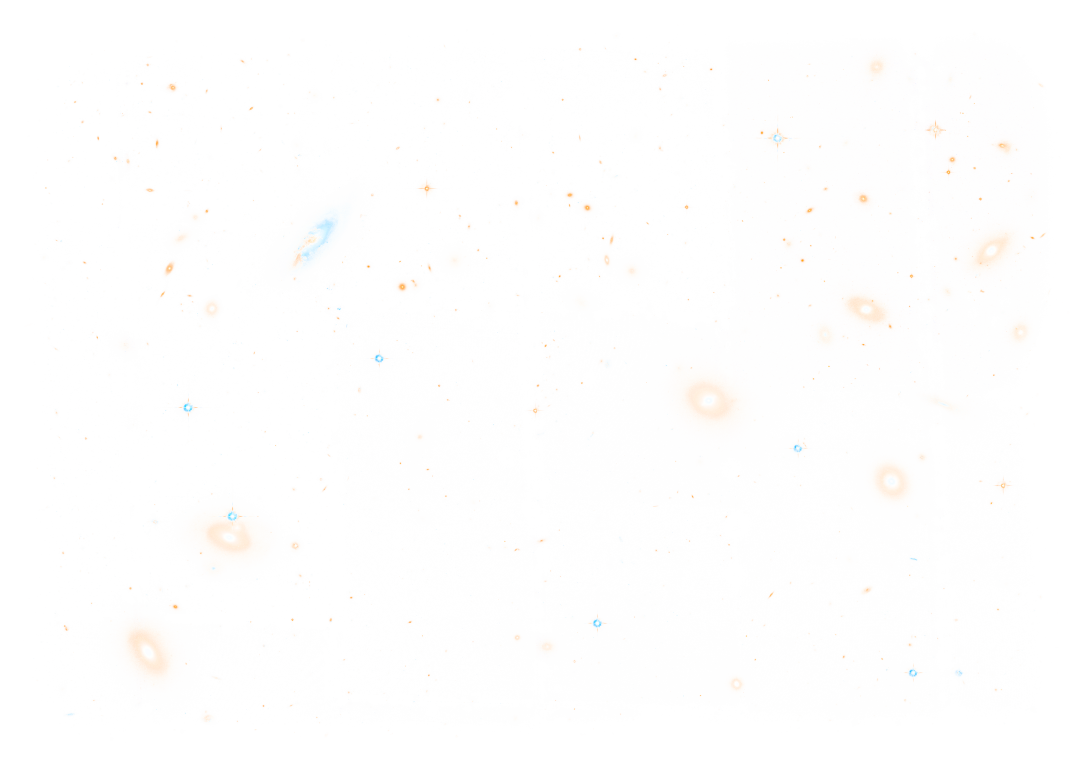
\includegraphics[width=8cm, angle=90]{coma_cluster_transparent_small.png}};
        \node[inner sep=0pt]
            at (galaxy) {
                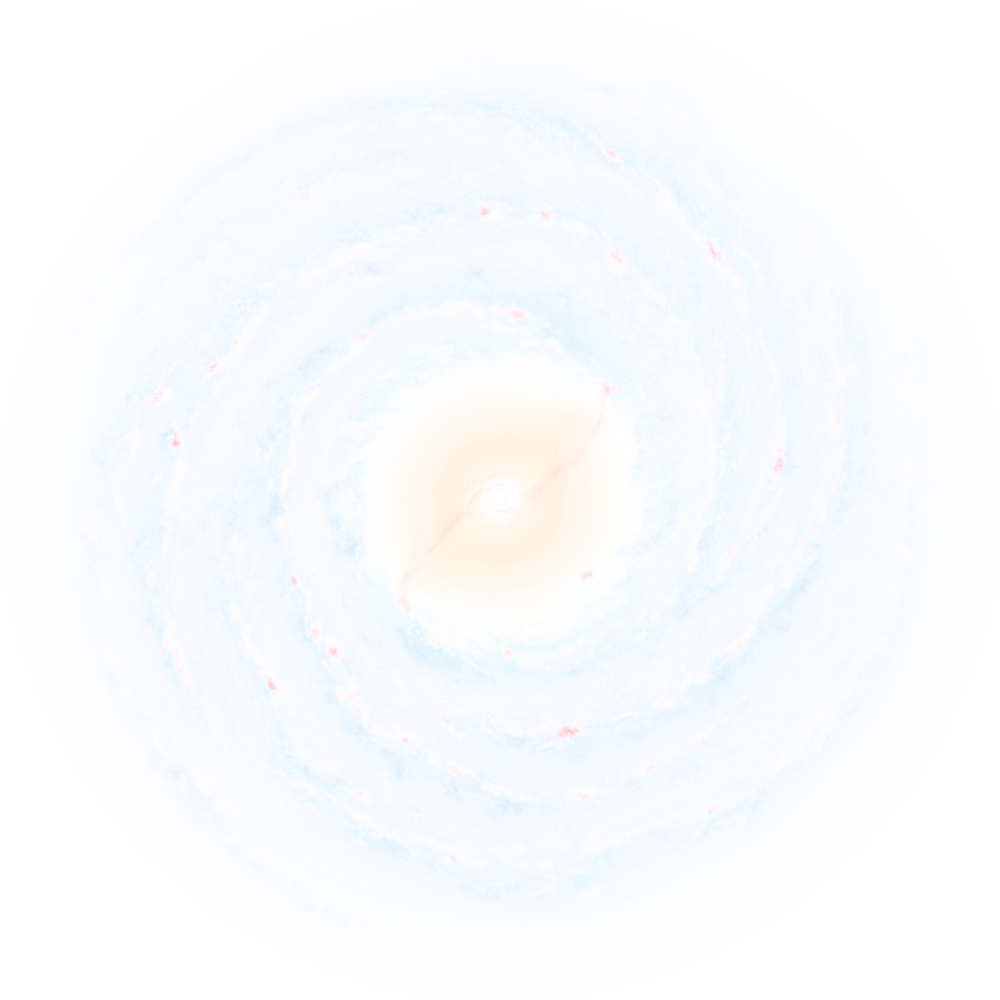
\includegraphics[width=8cm, angle=90]{
                    milky_way_2_transparent_small.png}};

        \foreach \r / \angle in {1.5/-125, 2.5/-110, 3.5/-100}
        {
            \draw[speed arrow, visible on = <1>]
                (galaxy) +(-90:\r)
                arc [
                    radius = \r,
                    start angle = -90,
                    end angle = \angle];
        }
        \foreach \r in {1.5, 2.5, 3.5}
        {
            \draw[speed arrow, visible on = <2->]
                (galaxy) +(-90:\r)
                arc [
                    radius = \r,
                    start angle = -90,
                    end angle = -120];
        }
        %\node[inner sep=0pt] (galaxy) at (8cm,2cm) {\includegraphics[width=6cm{bullet_cluster_transparent_small.png}};
        \begin{axis}[
            at = {(5cm,-1cm)},
            axis x line = bottom,
            axis y line = left,
            width = 7cm,
            height = 4cm,
            xmin = 0,
            xmax = 16,
            ymin = 0,
            ymax = 160,
            xtick = \empty,
            ytick = \empty,
            xlabel style = {font = \scriptsize},
            ylabel style = {font = \scriptsize},
            xlabel = {Etäisyys keskustasta},
            ylabel = {Pyörimisnopeus},
            every axis plot/.append style = {very thick}
        ]
            \addplot+ [visible on = <1->]
                table [col sep = comma] {rotation_visible.csv}
                node [sloped, above, pos = 0.95, font = \scriptsize] {odotus};
            \addplot+ [visible on = <2->]
                table [col sep = comma] {rotation_dark.csv}
                node [sloped, above, pos = 0.95, font = \scriptsize] {mitattu};
        \end{axis}
    \end{tikzpicture}
    \frametitle{Galaksien pyörimisnopeudet}
\end{frame}

\begin{frame}
    \frametitle{Pimeä aine Maan läheisyydessä}
    \nothing{
    \begin{itemize}
        \item Linnunrata lepää pimeästä aineesta koostuvan pilven keskellä
        \item Aurinko kiertää Linnunradan keskusta noin 230 km/s
        \item Maa kiertää Aurinkoa noin 30 km/s
        \item Maahan osuu jakuvasti pimeän aineen ``tuuli'', jonka nopeus vaihtelee vuoden ympäri Maan liikeradan vuoksi
        \item Maasta katsottuna tuuli tulee Joutsenen tähtikuvion suunnalta
    \end{itemize}
    }
    \nothing {
    \begin{itemize}
        \item Maan läpi kulkee noin 16 grammaa pimeää ainetta joka sekunti
        \item Maan liikkeen takia maahan osuvan pimeän aineen määrä vaihtelee vuoden ympäri
        \item Vuotuinen vaihtelu yksi tärkeimmistä todisteista mahdollisesta pimeän aineen löydöstä
    \end{itemize}
    }
    \begin{tikzpicture}[
        guide line/.style = {color = white!30!transparent, thin},
        speed arrow/.style = {very thick, -stealth},
        pointer arrow/.style = {very thick, -stealth},
        dm wind a/.style = {
            thick,
            decorate,
            decoration = {
                snake,
                segment length = 1cm,
                amplitude = 0.8mm},
            -stealth
        },
        dm wind b/.style = {
            thick,
            decorate,
            decoration = {
                snake,
                segment length = 1.2cm,
                amplitude = 0.8mm},
            -stealth
        }
    ]
        % panel 1
        \coordinate (dm halo) at (0,0);
        \begin{scope}[visible on = <1->]
            \shade[
                    shading = radial,
                    inner color = scp-purple-dark-2!80!\defaultbgcolor,
                    outer color = \defaultbgcolor]
                (dm halo) circle [radius = 2.0cm];
            \node[inner sep = -5pt]
                (smol mw) at (dm halo) {
                    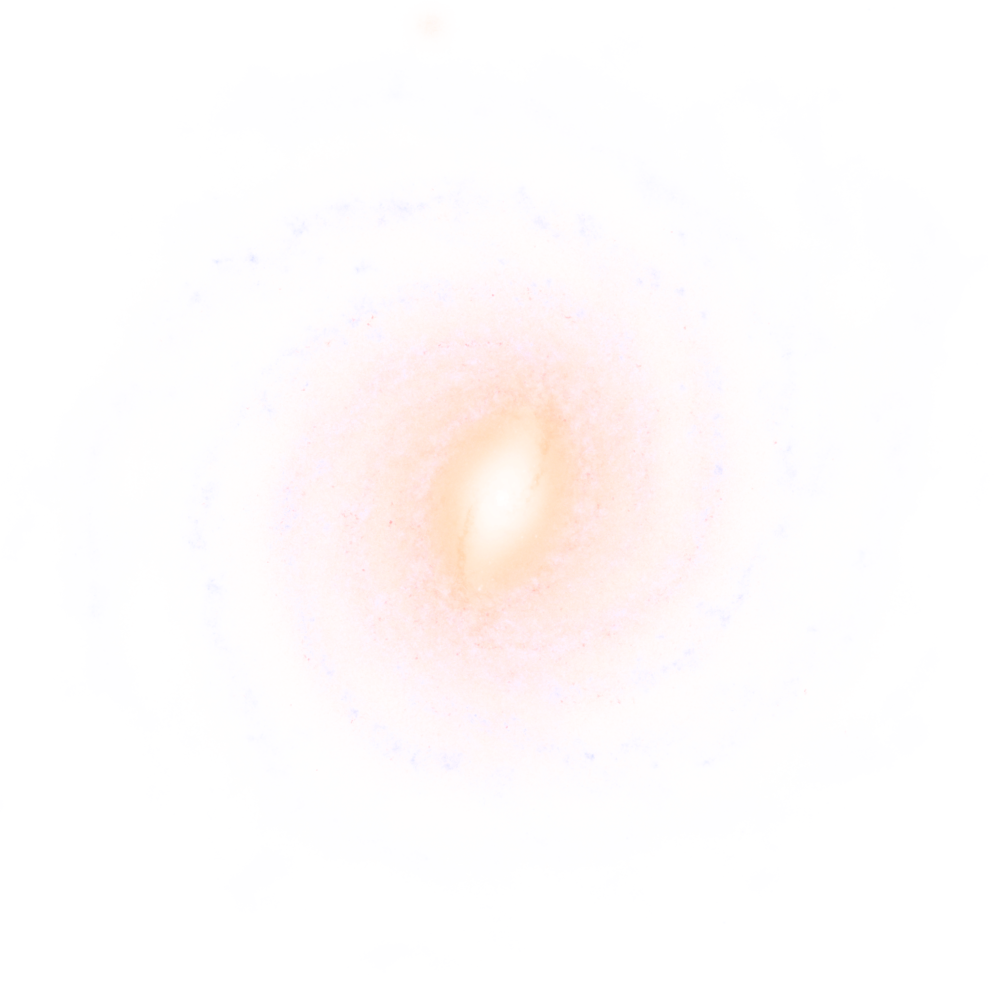
\includegraphics[width = 1.5cm]{
                        milky_way_transparent_crop_small.png}};
            \node
                at ($(dm halo) + (0, 1.2cm)$) [font = \scriptsize] {
                    Pimeää ainetta};
            \node
                (mw annot) at ($(dm halo) + (-1.5cm, -1cm)$) [
                        font = \scriptsize] {
                    Linnunrata};
            \draw[pointer arrow] (mw annot) to [out = 90, in = 180] (smol mw);
        \end{scope}

        % panel 2
        \coordinate (milky way) at (6cm,0);
        \begin{scope}[visible on = <2->]
            \node[inner sep = -10pt] at (milky way) {
                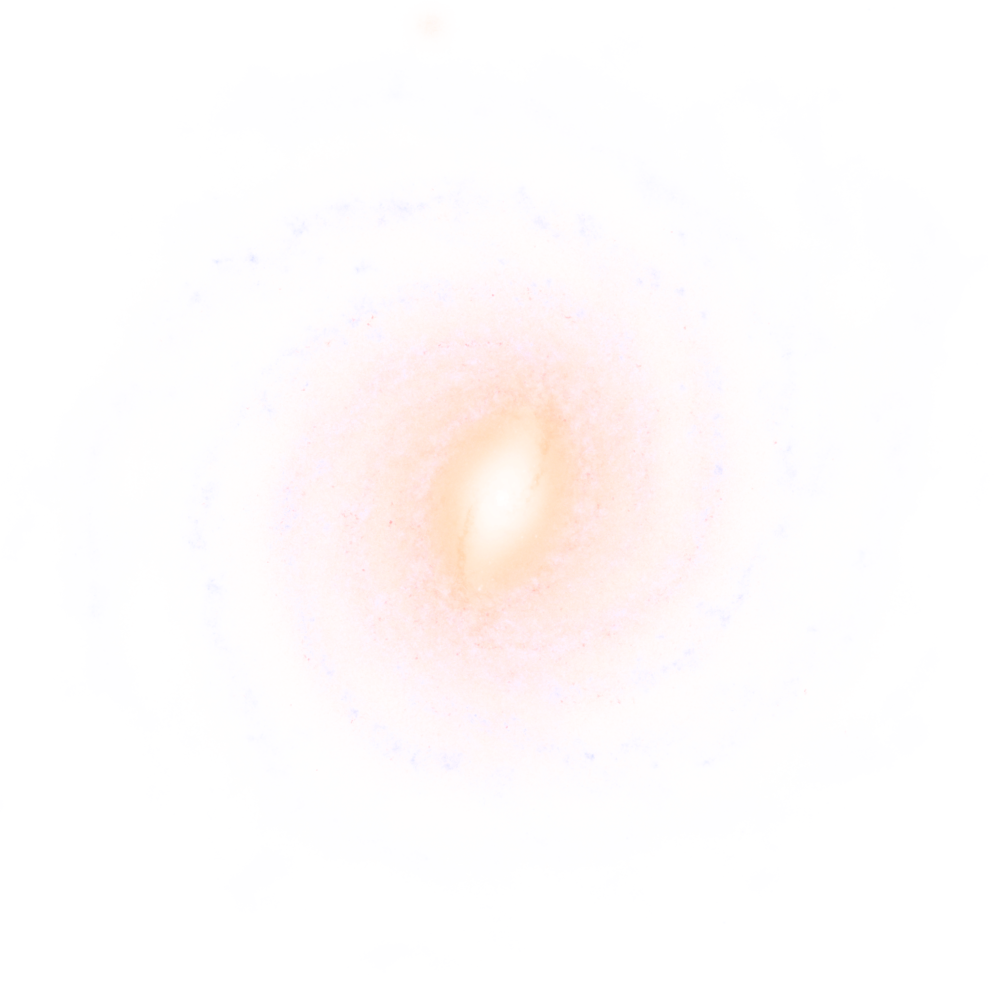
\includegraphics[width = 5cm]{
                    milky_way_transparent_crop_small.png}};
            \draw[speed arrow]
                (milky way) +(-90:0.8cm)
                arc [
                    start angle = -90,
                    end angle = -170,
                    radius = 0.8cm];
            \draw[
                    transparent,
                    decorate,
                    decoration = {
                        text along path,
                        text = {|\scriptsize\color{\defaulttextcolor}|230 km/s},
                        reverse path}]
                ($(milky way) + (-75:1.2cm)$)
                arc [
                    start angle = -75,
                    end angle = -155,
                    radius = 1.2cm];
            \draw[guide line] (dm halo) circle [radius = 0.4cm];
            \draw[guide line] (milky way) circle [radius = 1.7cm];
            \draw[guide line]
                ($(milky way) + (110:1.7cm)$) -- ($(dm halo) + (110:0.4cm)$);
            \draw[guide line]
                ($(milky way) + (-110:1.7cm)$) -- ($(dm halo) + (-110:0.4cm)$);
        \end{scope}
        
        % panel 3
        \coordinate (sun) at (6cm,-4cm);
        \begin{scope}[visible on = <3->]
            \node[inner sep = 0pt] at (sun) {
                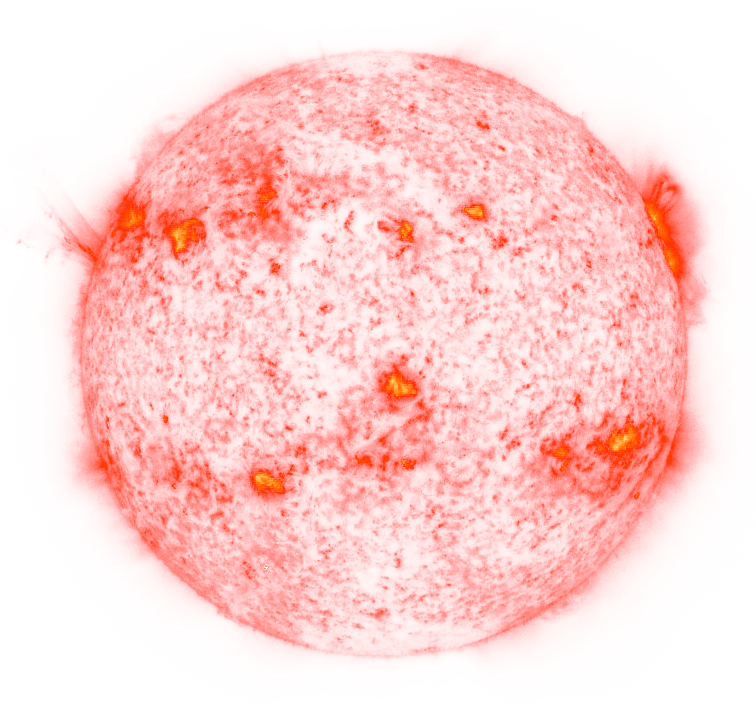
\includegraphics[width = 0.8cm]{sun_transparent.png}};
            \draw[very thin, white!30!transparent]
                (sun) circle [radius = 1.3cm];
            \draw[speed arrow]
                (sun) +(105:1.7cm)
                arc [
                    radius = 1.7cm,
                    start angle = 105,
                    end angle = 75]
                node [above, pos = 0.5, font = \scriptsize] {30 km/s};
            \draw[speed arrow]
                (sun) +(-75:1.7cm)
                arc [
                    radius = 1.7cm,
                    start angle = -75,
                    end angle = -105];
            \node[inner sep = 0pt]
                (earth down) at ($(sun) + (-90:1.3cm)$) {
                    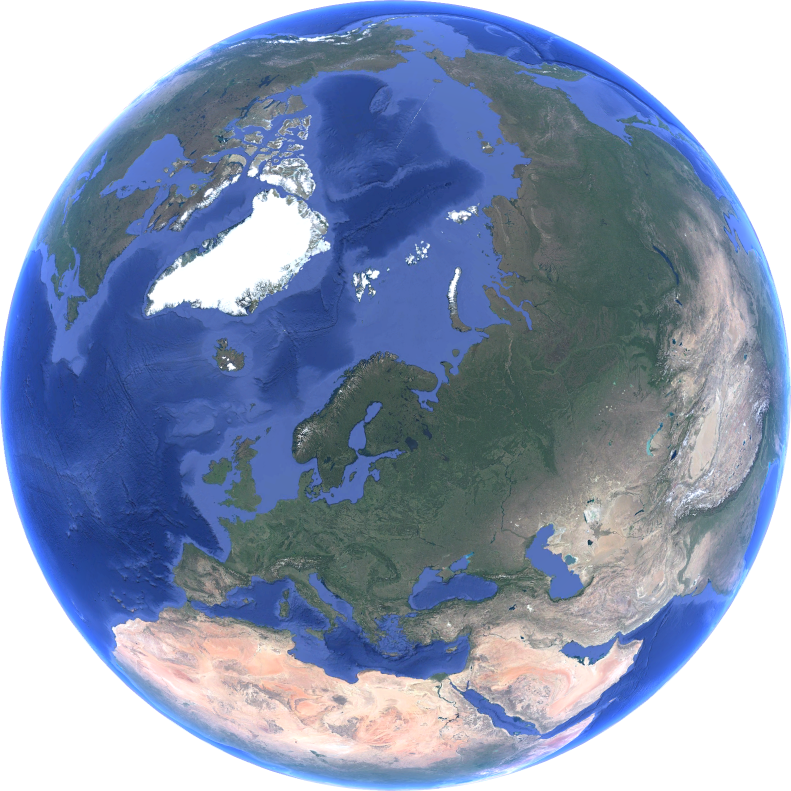
\includegraphics[width = 0.5cm]{
                        earth_transparent_small.png}};
            \node[inner sep = 0pt]
                (earth up) at ($(sun) + (90:1.3cm)$) {
                    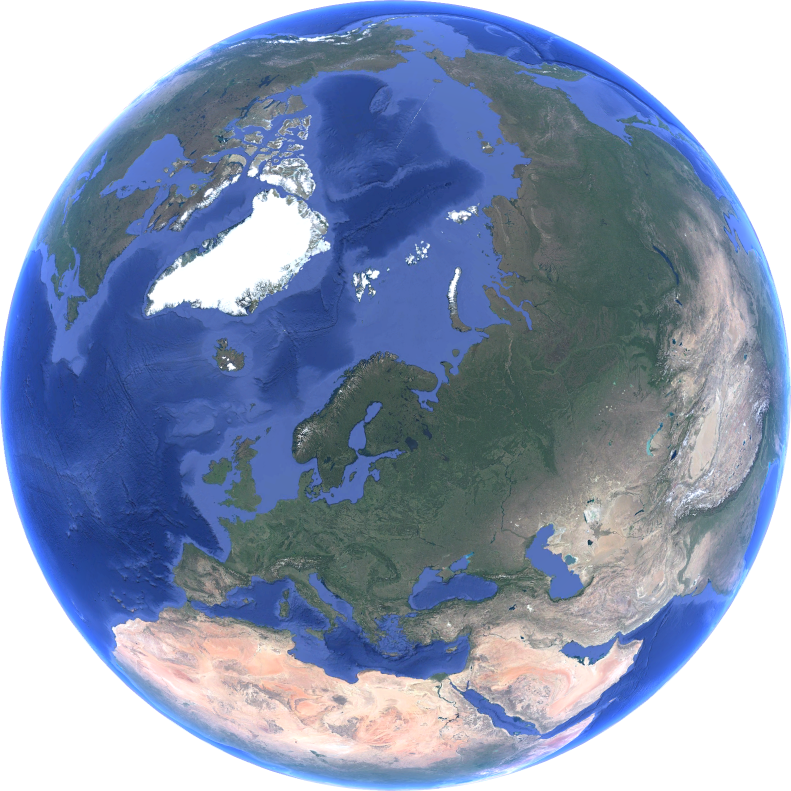
\includegraphics[width = 0.5cm]{
                        earth_transparent_small.png}};
            \draw[guide line] (sun) circle [radius = 1.7cm];
            \draw[guide line]
                ($(milky way) + (-90:1cm)$) -- ($(sun) + (140:1.7cm)$);
            \draw[guide line]
                ($(milky way) + (-90:1cm)$) -- ($(sun) + (40:1.7cm)$);
        \end{scope}
        
        % panel 4
        \coordinate (earth) at (0cm,-4cm);
        \begin{scope}[visible on = <4->]
            \node[inner sep = 0pt] at (earth) {
                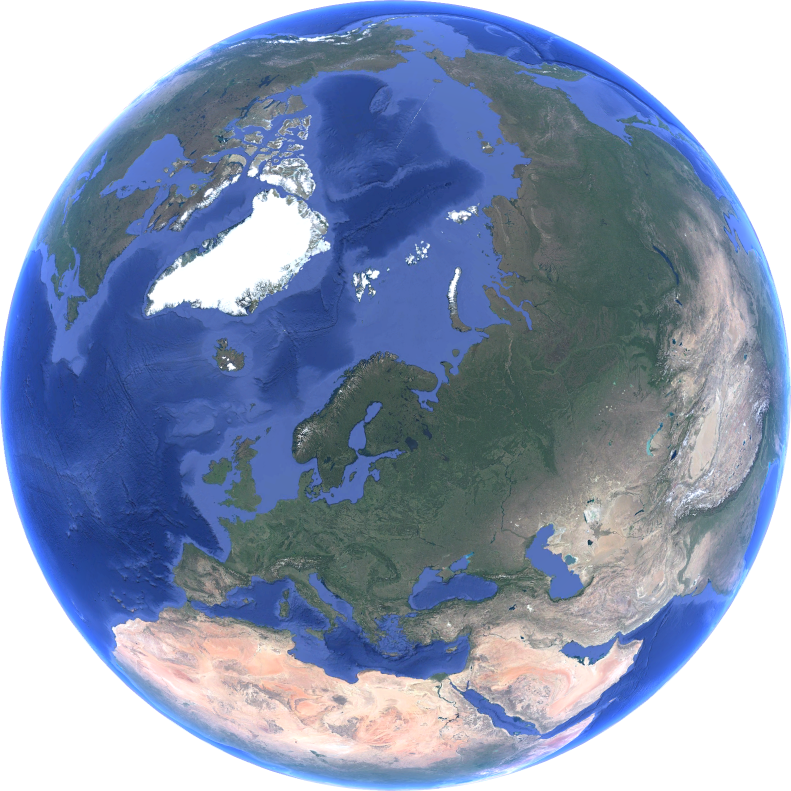
\includegraphics[width = 2.4cm]{earth_transparent_small.png}};

            \node
                at ($(earth) + (-2.0cm,0.99)$) [
                        above = 0.2cm,
                        font = \scriptsize] {
                    Pimeän aineen tuuli};
            \draw[dm wind b, -stealth]
                ($(earth) + (-3.0cm,-0.99)$) -- +(2.1cm,0);
            \draw[dm wind a, -stealth]
                ($(earth) + (-3.0cm,-0.33)$) -- +(1.75cm,0);
            \draw[dm wind a, -stealth]
                ($(earth) + (-3.0cm,0.33)$) -- +(1.75cm,0);
            \draw[dm wind b, -stealth]
                ($(earth) + (-3.0cm,0.99)$) -- +(2.1cm,0);
            \draw[guide line]
                (earth down) circle [radius = 0.4cm];
            \draw[guide line]
                (earth) circle [radius = 1.6cm];
            \draw[guide line]
                ($(earth down) + (90:0.4cm)$) -- ($(earth) + (60:1.6cm)$);
            \draw[guide line]
                ($(earth down) + (-90:0.4cm)$) -- ($(earth) + (-90:1.6cm)$);
        \end{scope}

    \end{tikzpicture}
\end{frame}

\begin{frame}
    \frametitle{Pimeän aineen tuuli}
    \nothing{
        \begin{itemize}
            \item Pimeä aine tulee maata kohti Joutsenen tähdistön suunnalta
        \end{itemize}
    }
    \begin{tikzpicture}[
        small circle/.style = {radius = 1pt},
        constellation/.style = {
            mark = *,
            mark color = white,
            color = white},
        grid line/.style = {
            mark = none,
            solid,
            color = black!80!white}
    ]
        \begin{axis}[
            axis equal image,
            axis lines = none,
            width = 16cm,
            height = 8cm,
            xmin = -2,
            xmax = 2,
            ymin = 0,
            ymax = 2,
            xtick = \empty,
            ytick = \empty
        ]
            \addplot [visible on = <2->, opacity = 0.7]
                graphics [xmin=-2,xmax=2,ymin=-2,ymax=2] {
                    directional_scatter_SHM_0.5GeV_2025-03-06-21-00-00_transparent.png};

            \addplot+ [grid line]
                table {star_map/horizontal_line_0.dat};
            \addplot+ [grid line]
                table {star_map/horizontal_line_1.dat};
            \addplot+ [grid line]
                table {star_map/horizontal_line_2.dat};
            \addplot+ [grid line]
                table {star_map/horizontal_line_3.dat};
            \addplot+ [grid line]
                table {star_map/horizontal_line_4.dat};
            \addplot+ [grid line]
                table {star_map/vertical_line_0.dat};
            \addplot+ [grid line]
                table {star_map/vertical_line_1.dat};
            \addplot+ [grid line]
                table {star_map/vertical_line_2.dat};
            \addplot+ [grid line]
                table {star_map/vertical_line_3.dat};
            \addplot+ [grid line]
                table {star_map/vertical_line_4.dat};
            \draw[color = black!80!white] (0,0) circle [radius=2];

            \addplot+ [constellation]
                table {star_map/constellation_Cygnus_2025-03-06-21-00.dat}
                node [
                        pos = 0.5,
                        left = 1mm,
                        anchor = east,
                        color = \defaulttextcolor,
                        font = \tiny] {
                    Joutsen};
            \addplot+ [constellation]
                table {star_map/constellation_Ursa-Major_2025-03-06-21-00.dat} 
                node [
                        pos = 0.5,
                        right = 1mm,
                        anchor = west,
                        color = \defaulttextcolor,
                        font = \tiny] {
                    Otava};
            \addplot+ [constellation]
                table {star_map/constellation_Ursa-Minor_2025-03-06-21-00.dat} 
                node [
                        pos = 0.5,
                        below = 1mm,
                        anchor = north,
                        color = \defaulttextcolor,
                        font = \tiny] {
                    Pieni Otava};
            \addplot+ [
                    mark = *,
                    mark size = 1mm,
                    color = scp-orange-dark-1,
                    opacity = 1.0]
                table {star_map/vlab_2025-03-06-21-00.dat}
                node (dm wind) {};
            \node[visible on = <1>]
                (annot) at (0,0.5) [
                        align = center,
                        left,
                        font = \footnotesize] {
                    Maan liikkeen suunta\\ galaksin suhteen};
            \draw[visible on = <1>, -stealth]
                (annot) to [out = 0, in = 90] (dm wind);
        \end{axis}
    \end{tikzpicture}
\end{frame}

\tikzset
{
    pics/proton/.style = {
        code = {
            \shade[ball color = proton-red] circle [radius = 0.3];
        }
    },
    pics/neutron/.style = {
        code = {
            \shade[ball color = white] circle [radius = 0.3];
        }
    },
    pics/nucleus/.style = {
        code = {
            \begin{scope}[transform shape]
                \pic at (113.90:0.6676) {proton};
                \pic at (-177.89:0.6676){proton};
                \pic at (40.41:0.6676) {proton};
                \pic at (-21.08:0.6676) {proton};
                \pic at (-53.65:0.6218) {neutron};
                \pic at (-98.08:0.6676) {proton};
                \pic at (8.77:0.6218) {neutron};
                \pic at (85.01:0.6735) {neutron};
                \pic at (144.30:0.6865) {neutron};
                \pic at (-143.41:0.7038) {neutron};
                \pic at (39.16:0.3022) {neutron};
                \pic at (-124.90:0.2973) {neutron};
                \pic at (132.23:0.3037) {proton};
                \pic at (-29.05:0.2774) {proton};
            \end{scope}
        }
    },
    pics/electron/.style = {
        code = {
            \shade[ball color = yellow!80!white] circle [radius = 0.3];
            %\draw (0,0) circle [radius = 0.5mm];
            \draw[black] (-0.2,0) -- (0.2,0);
        }
    },
    photon/.style = {
        thick,
        decorate,
        decoration = {
            snake,
            segment length = 1.8mm,
            amplitude = 0.8mm,
            post = lineto,
            post length = 1mm},
        -stealth
    }
}

\tikzfading[
    name = electron cloud, inner color = transparent!60, outer color = transparent!100]

\begin{frame}
    \frametitle{Pimeän aineen sironta}
    \nothing{
    \begin{itemize}
        \item Pimeä aine vuorovaikuttaa erittäin heikosti tavallisen aineen kanssa
        \item Satunnaisesti pimeä aine siroaa atomeista
        \item Pimeän aineen havaitseminen vaatii suuren määrän atoimeita, joista havaittujen sirontojen energia voidaan laskea
        \item Havaitsemiseen usitea teknologioita (skintillaatio, ionisaatio, lämpö)
        \item Kohdemateriaali vaikuttaa sirontaan
        \begin{itemize}
            \item Mitä suurempi massa, sitä todennäköisempää sironta
            \item Toisaalta mitä suurempi massa, sitä vähemmän energiaa siirtyy ytimelle
        \end{itemize}
    \end{itemize}
    }
    \begin{tikzpicture}[
        scatter arrow/.style = {thick, -stealth}
    ]
        \begin{scope}
            \coordinate
                (atom1) at (0,0);
            \coordinate
                (atom2) at (0,-3);
            
            % electron clouds
            \fill[
                visible on = <2->,
                yellow!80!white,
                path fading = electron cloud]
            (atom2) circle [radius=3.0cm];
            \fill[visible on = <1>, \defaultbgcolor]
                (atom2) circle [radius = 3.0cm];
            \fill[
                    visible on = <1->,
                    yellow!80!white,
                    path fading = electron cloud]
                (atom1) circle [radius=3.0cm];
            \fill[visible on = <1>, \defaultbgcolor]
                (atom1) circle [radius = 3.0cm];
            
            % nuclei
            \node[visible on = <1->, circle, minimum size = 1.0cm]
                (atom1 node) at (atom1) {}
                pic [scale = 0.4] {nucleus};
            \node[visible on = <2->, circle, minimum size = 1.0cm]
                (atom2 node) at (atom2) {}
                pic [visible on = <2->, shift = {(atom2)}, scale = 0.4] {nucleus};
            
            % annotations
            \node[visible on = <2->]
                at (-2.0cm,0) [font = \scriptsize] {
                    elektronipilvi};
            \node[visible on = <1->]
                at (0,0) [
                        right = 0.3cm,
                        font = \scriptsize,
                        anchor = west] {
                    atomiydin};
                
            % dm
            \node[visible on = <1->, circle, ball color = black!70!white]
                (dm) at (145:3.0cm) {};
            \node[visible on = <1->]
                at (145:3.0cm) [above right, font = \scriptsize] {
                    pimeä aine};
            
            \draw[visible on = <1->, scatter arrow]
                (35:3.0cm) -- (atom1 node.north) -- (dm);
            \draw[visible on = <1->, scatter arrow]
                (atom1 node.south) -- (atom2 node.north);
            \coordinate
                (ionize base) at ($(atom1) + (1.0,-1.5)$);
            \node[visible on = <3->, circle, minimum size=0.3cm]
                (ionize) at ($(ionize base) + (-10:1)$) {};
            \pic at (ionize) [visible on = <3->, very thick, scale = 0.4] {
                    electron};
            \draw[visible on = <3->, scatter arrow]
                (ionize base) -- (ionize);
                
            \node[visible on = <3->]
                at (ionize) [below right, font = \scriptsize] {
                    elektroni};
            \coordinate
                (light base) at ($(atom1) + (-0.9,-1.6)$);
            \draw[visible on = <4->, photon]
                (light base) -- +(-170:1)
                node [above, sloped, pos = 0.5, font = \scriptsize] {
                    valoa};
        \end{scope}
        \begin{axis}[
            visible on = <5->,
            at = {(4cm,-0.5cm)},
            width = 8cm,
            height = 4cm,
            xmin = -0.1,
            xmax = 1.2,
            ymin = -0.2,
            ymax = 1.2,
            xlabel = {Atomin massa},
            axis x line = bottom,
            axis y line = left,
            xtick = \empty,
            ytick = \empty,
            every plot/.append style = {very thick}
        ]
            \addplot+ [\defaulttextcolor, -stealth]
                coordinates { (0,0.6) (1,1) }
                node [sloped, pos = 0.5, above, font = \scriptsize] {
                    Sironnan todennäköisyys};
            \addplot+ [\defaulttextcolor, -stealth]
                coordinates { (0,0.4) (1,0) }
                node [sloped, pos = 0.5, below, font = \scriptsize]{
                    Energia};
        \end{axis}
        \begin{axis}[
            visible on = <6->,
            at = {(4cm,-3.0cm)},
            width = 8cm,
            height = 3cm,
            xmin = -0.1,
            xmax = 1.2,
            ymin = -0.2,
            ymax = 1.2,
            xlabel = {Pimeän aineen massa},
            axis x line = bottom,
            axis y line = left,
            xtick = \empty,
            ytick = \empty,
            every plot/.append style = {very thick}
        ]
            \addplot+ [\defaulttextcolor, -stealth]
                coordinates { (0,0.0) (1,1) }
                node [sloped, pos = 0.5, below, font = \scriptsize]{
                    Energia};
        \end{axis}
    \end{tikzpicture}
\end{frame}

\nothing
{
\begin{frame}
    \frametitle{Pimeän aineen sironta}
    \begin{tikzpicture}
        \begin{scope}
            \shade[
                    shading = radial,
                    inner color = yellow!80!white!30!\defaultbgcolor,
                    outer color = \defaultbgcolor]
                (dm halo) circle [radius=3.0cm];
            \node[circle, minimum size=1.0cm]
                (atom) at (0,0) [right, font = \tiny] {
                    Atomiydin}
                pic [scale = 0.4] {
                    nucleus};
            \node[circle, ball color = black!70!white]
                (dm) at (135:3.5cm) [above right, font = \tiny] {
                    Pimeä aine};
            \draw[-stealth]
                (45:3.5cm) -- (atom.north) -- (dm);
            %\node[circle, minimum size=0.8cm] at (2,0) {} pic[scale = 0.3] {nucleus};
        \end{scope}
    \end{tikzpicture}
    \nothing
    {
    \begin{itemize}
        \item Kun pimeä aine siroaa atomiytimestä, osa energiasta siirtyy sitä ympäröivään elektronipilveen
        \item Jos elektroni saa tarpeeksi energiaa, se irtoaa atomista
        \item Elektronin irrottaminen vaatii jonkin verran energiaa
        \item Pienin havaittavissa oleva energia
        \item Suuntariippuvainen kristalleissa
        \item Aiheuttaa pävittäisen vaihtelun havaittavissa olevien sirontojen määrään
    \end{itemize}
    }
\end{frame}
}

\begin{frame}
    \frametitle{Pimeän aineen havaitseminen}
    \nothing{
        \begin{itemize}
            \item Viimeaikoina parhaiten menestyneet kokeet käyttävät nestemäistä xenon-jalokaasua
            \item Vaihtoehtona kiinteät kristalliset kohdemateriaalit
        \end{itemize}
    }
    \begin{tikzpicture} [
    ]
        % Xenon tank
        \begin{scope}[
            visible on = <1->,
            shift = {(0,0)}
        ]
            \node
                (xenon) at (0,0) {
                    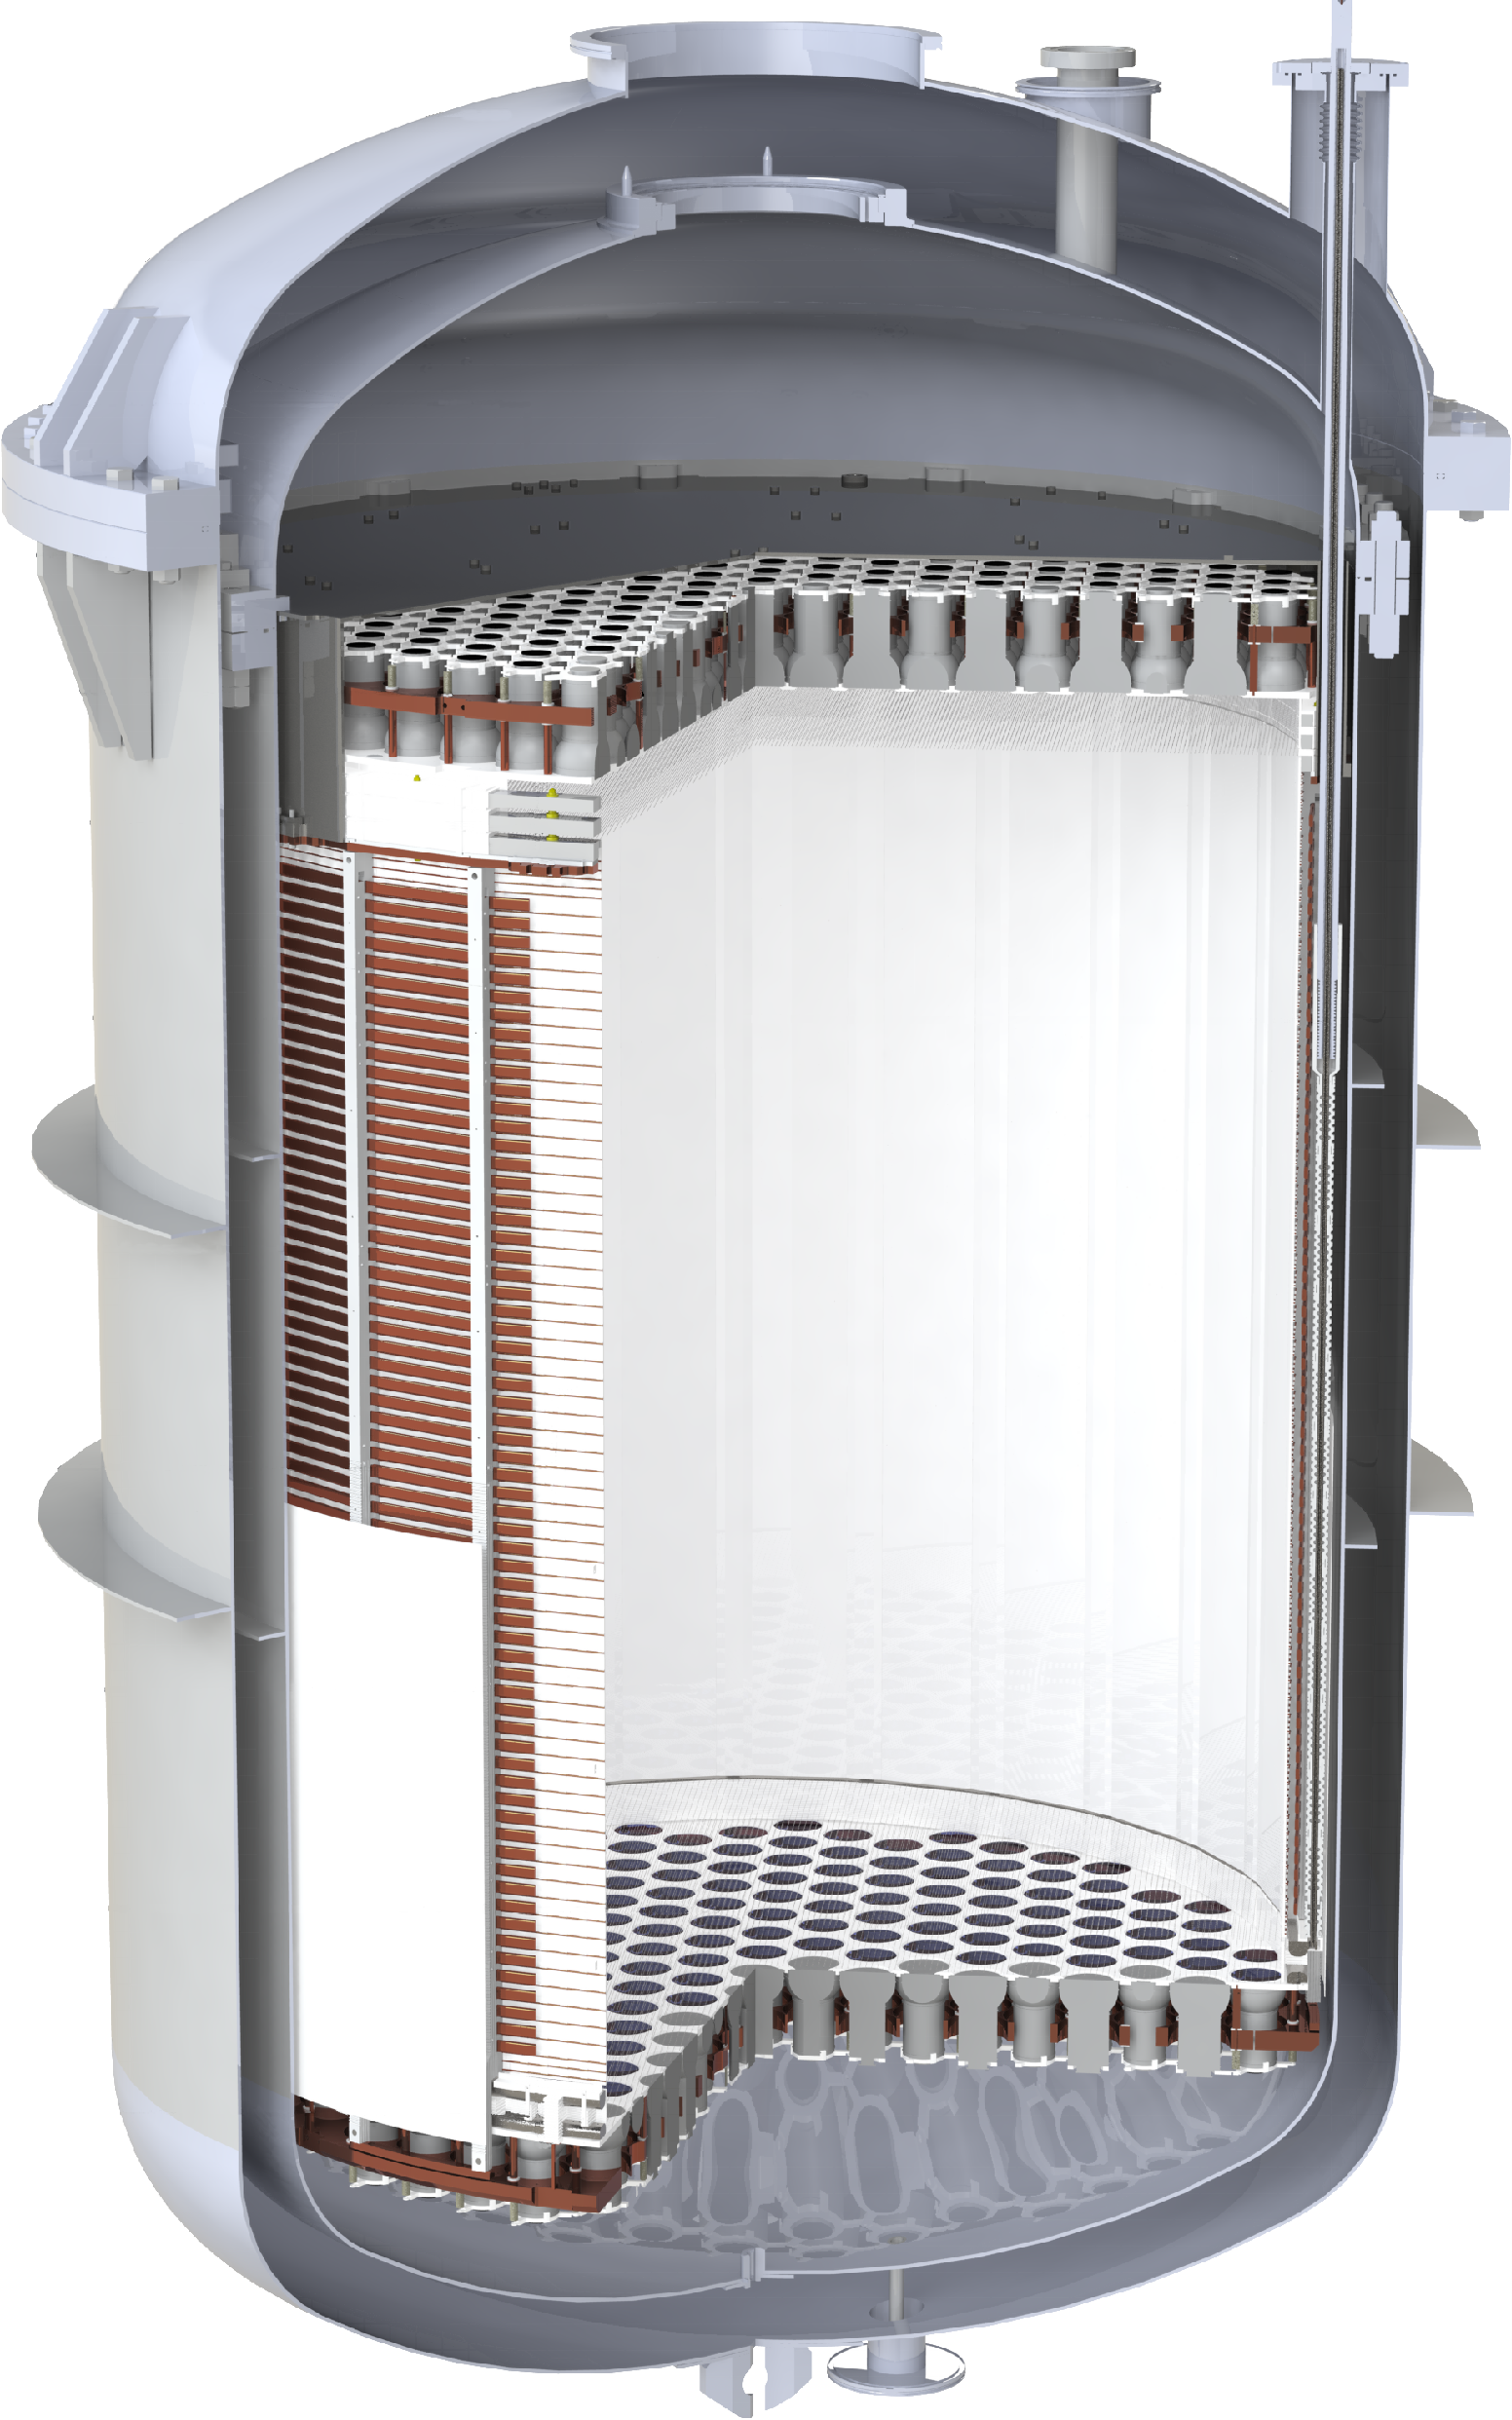
\includegraphics[width = 4cm]{
                        xenon_cryostat_render_fix.png}};
            \fill[scp-green-light-1, opacity = 0.3]
                (-0.400,1.156)
                -- ++(0.412,0.224)
                -- ++(1.434,-0.022)
                -- ++(-0.04,-3.412)
                -- ++(-1.400,0.044)
                -- ++(-0.399,-0.444)
                -- cycle;
            \foreach \i in {0, 1, 2, 3}
            {
                \pgfmathsetmacro{\xshift}{0.1 + \i*0.4}
                \pgfmathsetmacro{\topyshift}{3.204 + \i*0.012}
                \pgfmathsetmacro{\botyshift}{-1.9 - \i*0.018}
                \draw[black, stealth-]
                    (\xshift,\botyshift) -- ++(0,\topyshift);
            }
            \foreach \i in {0, 1, 2}
            {
                \pgfmathsetmacro{\xshift}{0.3 + \i*0.4}
                \pgfmathsetmacro{\topyshift}{1.2 - \i*0.006}
                \pgfmathsetmacro{\botyshift}{-1.9 - \i*0.018}
                \node
                    at (\xshift,\topyshift) [text = black, font = \tiny] {$+$};
                \node
                    at (\xshift,\botyshift) [text = black, font = \tiny] {$-$};
            }
            \node (annot) at ($(xenon) + (0,2.2)$) [
                    inner sep = 1pt,
                    align = center,
                    draw = black,
                    fill = white,
                    text opacity = 1,
                    fill opacity = 0.6,
                    font = \footnotesize,
                    text = \defaultbgcolor] {
                nestemäistä\\ jalokaasua};
            \draw[black, -stealth]
                (annot) to [out = -90, in = 90] (-0.15,1.0);
        \end{scope}

        % Germanium crystal
        \begin{scope}[
            visible on = <2->,
            shift = {(6.0cm,1.5cm)}
        ]
            \coordinate
                (crystal) at (0, 0);
            \node
                (germanium) at (crystal) {
                    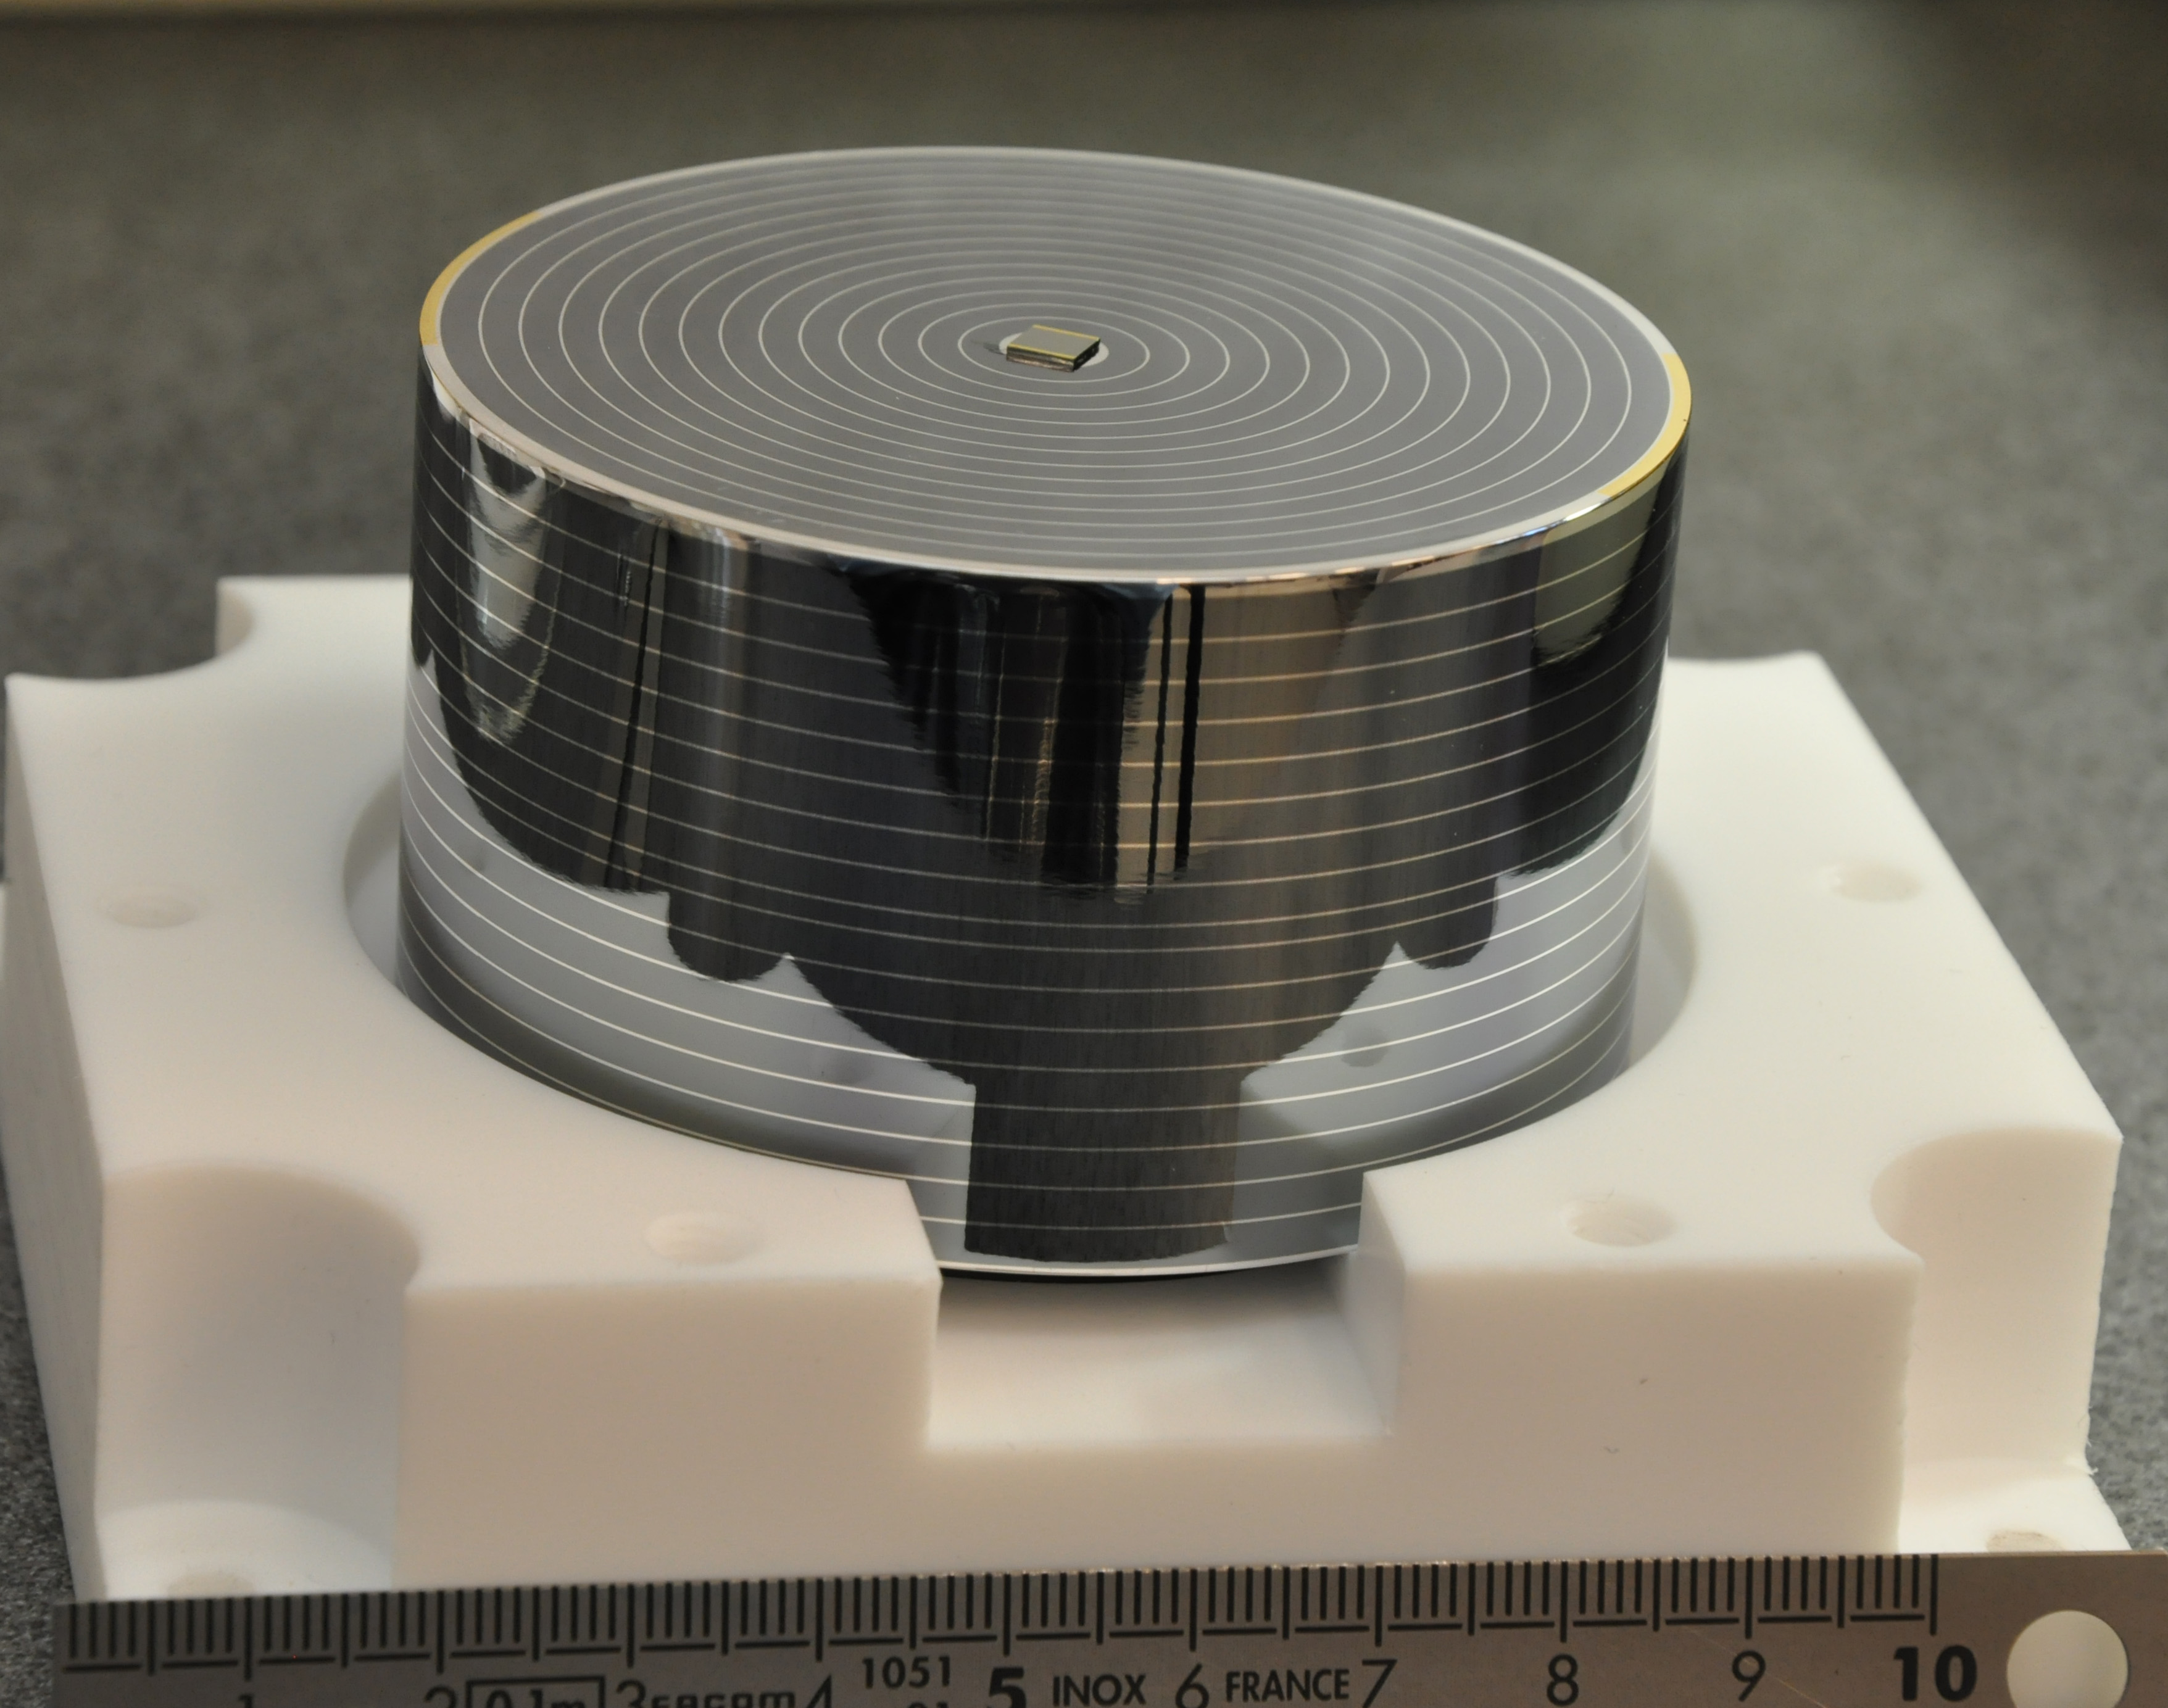
\includegraphics[
                            width = 6cm,
                            trim = {0 6cm 1cm 1.3cm},
                            clip] {
                        edelweiss_bolo.jpg}};
            \node
                at (crystal) [opacity = 0.8]{
                    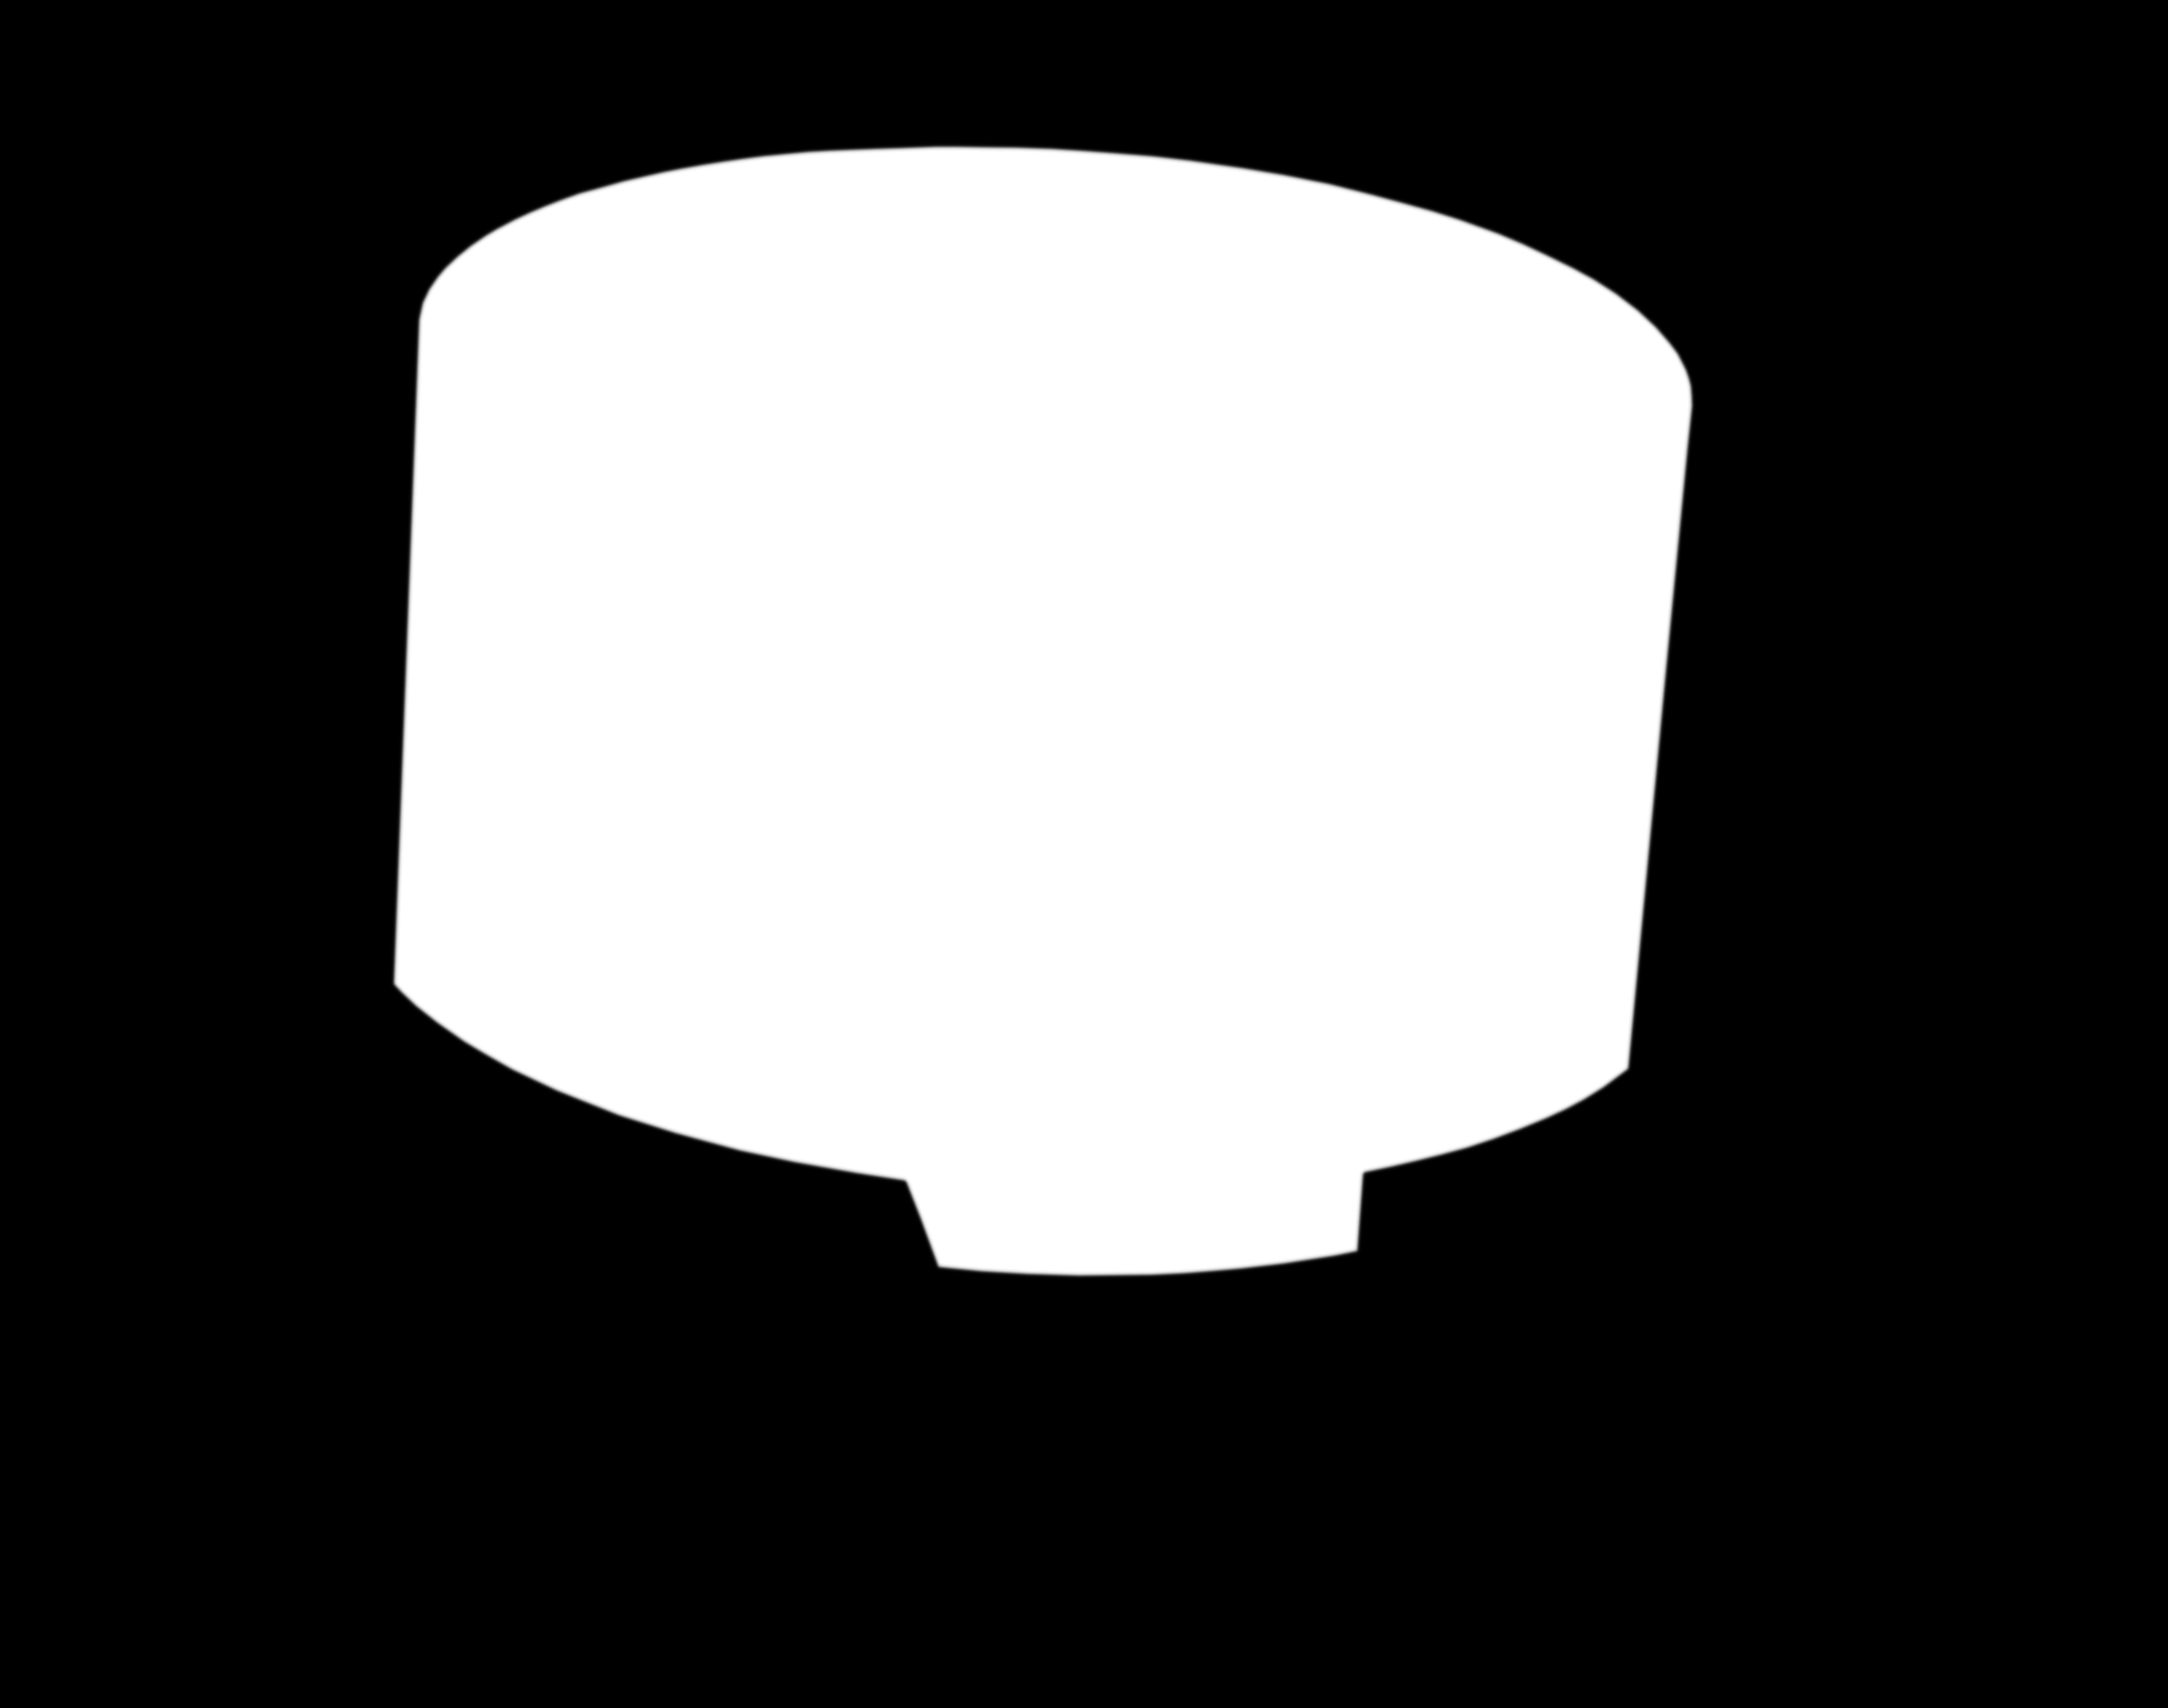
\includegraphics[
                            width = 6cm,
                            trim = {0 6cm 1cm 1.3cm},
                            clip] {
                        edelweiss_bolo_mask.png}};
            \node
                at (germanium) [above = 1.6cm] {
                    Germaniumkide};
        \end{scope}

        % Germanium cut
        \begin{scope}[
            visible on = <3->,
            shift = {(6.0cm,-1.5cm)},
            germanium block draw/.style = {draw = white},
            germanium block fill/.style = {fill = black!85!white},
        ]
            \fill[germanium block fill]
                (1.7,0) arc [
                    x radius = 1.7,
                    y radius = 0.85,
                    start angle = 0,
                    end angle = 240]
                -- (0,0) -- cycle;
            \fill[germanium block fill]
                (-1.7,0)
                arc [
                    x radius = 1.7,
                    y radius = 0.85,
                    start angle = 180,
                    end angle = 240]
                -- ++(0,-1.7)
                arc [
                    x radius = 1.7,
                    y radius = 0.85,
                    start angle = 240,
                    end angle = 180]
                -- cycle;
            \fill[germanium block fill]
                (0,0)
                -- (240:1.7 and 0.85)
                -- ++(0,-1.7)
                -- (0,-1.7)
                --cycle;
            \fill[germanium block fill]
                (0,0)
                -- ++(1.7,0)
                -- ++(0,-1.7)
                -- ++(-1.7,0)
                --cycle;
            \fill[white!50!black]
                (0.12,0)
                arc [
                    x radius = 0.12,
                    y radius = 0.06,
                    start angle = 0,
                    end angle = 230]
                -- (0,0)
                -- cycle;
            \foreach \i in {2,...,13}
            {
                \pgfmathsetmacro{\xradius}{\i*0.12}
                \pgfmathsetmacro{\yradius}{\i*0.06}
                \draw[thin, white!50!black]
                    (\xradius,0)
                    arc [
                        x radius = \xradius,
                        y radius = \yradius,
                        start angle = 0,
                        end angle = 240];
            }
            \foreach \i in {1,...,16}
            {
                \pgfmathsetmacro{\yshift}{\i*-0.1}
                \draw[thin, white!50!black]
                    (-1.7,\yshift)
                    arc [
                        x radius = 1.7,
                        y radius = 0.85,
                        start angle = 180,
                        end angle = 240];
            }
            \draw[germanium block draw]
                (-1.7,0)
                arc [
                    x radius = 1.7,
                    y radius = 0.85,
                    start angle = 180,
                    end angle = 240]
                -- ++(0,-1.7)
                arc [
                    x radius = 1.7,
                    y radius = 0.85,
                    start angle = 240,
                    end angle = 180]
                -- cycle;
            \draw[germanium block draw]
                (0,0)
                -- (240:1.7 and 0.85)
                -- ++(0,-1.7)
                -- (0,-1.7)
                --cycle;
            \draw[germanium block draw]
                (0,0)
                -- ++(1.7,0)
                -- ++(0,-1.7)
                -- ++(-1.7,0)
                --cycle;
            \draw[germanium block draw]
                (1.7,0)
                arc [
                    x radius = 1.7,
                    y radius = 0.85,
                    start angle = 0,
                    end angle = 240]
                -- (0,0)
                -- cycle;
            \fill[fill = yellow!50!gray]
                (1.7,0)
                arc [
                    x radius = 1.7,
                    y radius = 0.85,
                    start angle = 0,
                    end angle = 240]
                -- (240:1.65 and 0.825)
                arc [
                    x radius = 1.65,
                    y radius = 0.825,
                    start angle = 240,
                    end angle = 0]
                -- cycle;

            \foreach \i in {1, 2, 3}
            {
                \pgfmathsetmacro{\xshift}{\i*0.425}
                \draw[white, -stealth] (\xshift,-0.1) -- ++(0,-1.5);
            }
            \foreach \i in {0, 1, 2, 3}
            {
                \pgfmathsetmacro{\xshift}{0.2125 + \i*0.425}
                \node at (\xshift,-0.2) [text = white, font = \tiny] {$+$};
                \node at (\xshift,-1.5) [text = white, font = \tiny] {$-$};
            }
        \end{scope}
    \end{tikzpicture}
\end{frame}

\begin{frame}
    \frametitle{Kidevirheet}
    \begin{tikzpicture}[
        background atom/.style = {ball color = scp-blue-light-2},
        hit atom/.style = {ball color = scp-blue-dark-1},
        graph line/.style = {very thick},
        scatter arrow/.style = {thick, -stealth},
        graph arrow/.style = {very thick, -stealth}
    ]
        % frame 1
        \begin{scope}[
            visible on = <1->,
            shift = {(0,0)}
        ]
            \node[circle]
                (atom1) at (0.75, 0.75) {};
            \node[visible on = <2->, circle, ball color = black!70!white]
                (dm1) at (-0.75, 0.3) {};
            \draw[visible on = <2->, scatter arrow]
                (dm1) -- (atom1);
            \shade[hit atom]
                (atom1) circle [radius = 0.1cm];
            \foreach \x in {0, 1.5, 3.0}
                \foreach \y in {0, 1.5, 3.0}
                    \shade[background atom]
                        (\x,\y) circle [radius = 0.1cm];
            \shade[background atom]
                ($(0,1.5) + (0.75, 0.75)$) circle [radius = 0.1cm];
            \shade[background atom]
                ($(1.5,0) + (0.75, 0.75)$) circle [radius = 0.1cm];
            \shade[background atom]
                ($(1.5,1.5) + (0.75, 0.75)$) circle [radius = 0.1cm];
            \draw[graph arrow]
                (-0.2cm,-2.2cm)
                -- (-0.2cm,-0.5cm)
                node [sloped, pos = 0.5, above, font = \scriptsize] {
                    Energia};
            \begin{scope}[shift = {(0,-0.3cm)}]
                \shade[hit atom]
                    (0.75cm,-1.5cm) circle [radius = 0.1cm];
                \draw[graph line] (0,-0.6cm)
                    ..controls (1.05cm,-3.0cm) and (1.0cm,-0.5cm)
                    .. (1.69cm, -0.78cm)
                    ..controls (1.9cm,-0.9cm)
                    .. (2.25cm,-0.7cm);
            \end{scope}
        \end{scope}
        
        % frame 2
        \begin{scope}[
            visible on = <3->,
            shift = {(5.0,0)}
        ]
            \node[circle]
                (atom2) at (0.75, 0.75) {};
            \node[circle]
                (dm21) at (-0.75, 0.3) {};
            \node[circle, ball color = black!70!white]
                (dm22) at (-0.75, 1.2) {};
            \draw[scatter arrow]
                (dm21) -- (atom2.west) -- (dm22);
            \draw[scatter arrow]
                (atom2) +(0:0.15) -- ++(15:0.75);
            \shade[hit atom]
                (atom2) + (0.15,0) circle [radius = 0.1cm];
            \foreach \x in {0, 1.5, 3.0}
                \foreach \y in {0, 1.5, 3.0}
                    \shade[background atom]
                        (\x,\y) circle [radius = 0.1cm];
            \shade[background atom]
                ($(0,1.5) + (0.75, 0.75)$) circle [radius = 0.1cm];
            \shade[background atom]
                ($(1.5,0) + (0.75, 0.75)$) circle [radius = 0.1cm];
            \shade[background atom]
                ($(1.5,1.5) + (0.75, 0.75)$) circle [radius = 0.1cm];
            \begin{scope}[shift = {(0,-0.3cm)}]
                \shade[hit atom]
                    (0.9cm,-1.3cm) circle [radius = 0.1cm];
                \draw[graph line] (0,-0.6cm)
                    ..controls (1.05cm,-3.0cm) and (1.0cm,-0.5cm)
                    .. (1.69cm, -0.78cm)
                    ..controls (1.9cm,-0.9cm)
                    .. (2.25cm,-0.7cm);
            \end{scope}
        \end{scope}

        % frame 3
        \begin{scope}[
            visible on = <4->,
            shift = {(10.0,0)}
        ]
            \coordinate
                (atom31) at (0.75, 0.75) {};
            \coordinate
                (atom32) at (1.5, 1.5) {};
            \coordinate
                (atom33) at (2.25,2.25) {};
            \shade[hit atom]
                ($(atom31) + (1.125,1.125)$) circle [radius = 0.1cm];
            \foreach \x in {0, 1.5, 3.0}
                \foreach \y in {0, 1.5, 3.0}
                    \shade[background atom]
                        (\x,\y) circle [radius = 0.1cm];
            \shade[background atom]
                ($(0,1.5) + (0.75, 0.75)$) circle [radius = 0.1cm];
            \shade[background atom]
                ($(1.5,0) + (0.75, 0.75)$) circle [radius = 0.1cm];
            \shade[background atom]
                ($(1.5,1.5) + (0.75, 0.75)$) circle [radius = 0.1cm];
            \begin{scope}[shift = {(0,-0.3cm)}]
                \shade[hit atom]
                    (1.875cm,-0.7cm) circle [radius = 0.1cm];
                \draw[graph line] (0,-0.6cm)
                    ..controls (1.05cm,-3.0cm) and (1.0cm,-0.5cm)
                    .. (1.69cm, -0.78cm)
                    ..controls (1.9cm,-0.9cm)
                    .. (2.25cm,-0.7cm);
            \end{scope}
        \end{scope}
    \end{tikzpicture}
    \nothing
    {
        \begin{itemize}
            \item Ionisaatioon vaadittu sirontaenergia liitty läheisesti energiaan, joka vaaditaan siirtämään kristallin atomi pois paikoiltaan
            \item Väitöskirjassani tutkin tätä simuloimalla atomien liikettä pimeän aineen sironnan seurauksena
        \end{itemize}
    }
\end{frame}

\begin{frame}
    \frametitle{Virhe-energian suuntariippuvuus}
    \begin{tikzpicture}[
        grid line/.style = {
            mark = none,
            solid,
            color = black!80!white}
    ]
        \begin{axis}[
            axis equal image,
            axis lines = none,
            width = 16cm,
            height = 8cm,
            xmin = -2,
            xmax = 2,
            ymin = 0,
            ymax = 2,
            xtick = \empty,
            ytick = \empty
        ]
            \addplot
                graphics [xmin=-2, xmax=2, ymin=-2, ymax=2] {esurf_Ge.png};

            \addplot+ [grid line]
                table {star_map/horizontal_line_0.dat};
            \addplot+ [grid line]
                table {star_map/horizontal_line_1.dat};
            \addplot+ [grid line]
                table {star_map/horizontal_line_2.dat};
            \addplot+ [grid line]
                table {star_map/horizontal_line_3.dat};
            \addplot+ [grid line]
                table {star_map/horizontal_line_4.dat};
            \addplot+ [grid line]
                table {star_map/vertical_line_0.dat};
            \addplot+ [grid line]
                table {star_map/vertical_line_1.dat};
            \addplot+ [grid line]
                table {star_map/vertical_line_2.dat};
            \addplot+ [grid line]
                table {star_map/vertical_line_3.dat};
            \addplot+ [grid line]
                table {star_map/vertical_line_4.dat};
            \draw[color = black!80!white]
                (0,0) circle [radius=2];
        \end{axis}
    \end{tikzpicture}
\end{frame}

\begin{frame}
    \frametitle{Pimeän aineen tuuli kiteessä}
    \nothing{
        \begin{itemize}
            \item Pimeä aine tulee maata kohti Joutsenen tähdistön suunnalta
        \end{itemize}
    }
    \begin{tikzpicture}[
        small circle/.style = {radius = 1pt},
        constellation/.style = {
            mark = *,
            mark color = white,
            color = white},
        grid line/.style = {
            mark = none,
            solid,
            color = black!80!white}
    ]
        \begin{axis}[
            axis equal image,
            axis lines = none,
            width = 16cm,
            height = 8cm,
            xmin = -2,
            xmax = 2,
            ymin = 0,
            ymax = 2,
            xtick = \empty,
            ytick = \empty
        ]
            \addplot[visible on = <1>, opacity = 0.7]
                graphics [xmin=-2, xmax=2, ymin=-2, ymax=2] {
                    transparent_directional_event_SHM_0.5GeV_2025-03-06-21-00-00.png};
            \addplot[visible on = <2>, opacity = 0.7]
                graphics [xmin=-2, xmax=2, ymin=-2, ymax=2] {
                    transparent_directional_event_SHM_0.5GeV_2025-03-06-23-00-00.png};
            \addplot[visible on = <3>, opacity = 0.7]
                graphics [xmin=-2, xmax=2, ymin=-2, ymax=2] {
                    transparent_directional_event_SHM_0.5GeV_2025-03-07-00-59-59.png};
            \addplot[visible on = <4>, opacity = 0.7]
                graphics [xmin=-2, xmax=2, ymin=-2, ymax=2] {
                    transparent_directional_event_SHM_0.5GeV_2025-03-07-03-00-00.png};

            \addplot+ [grid line]
                table {star_map/horizontal_line_0.dat};
            \addplot+ [grid line]
                table {star_map/horizontal_line_1.dat};
            \addplot+ [grid line]
                table {star_map/horizontal_line_2.dat};
            \addplot+ [grid line]
                table {star_map/horizontal_line_3.dat};
            \addplot+ [grid line]
                table {star_map/horizontal_line_4.dat};
            \addplot+ [grid line]
                table {star_map/vertical_line_0.dat};
            \addplot+ [grid line]
                table {star_map/vertical_line_1.dat};
            \addplot+ [grid line]
                table {star_map/vertical_line_2.dat};
            \addplot+ [grid line]
                table {star_map/vertical_line_3.dat};
            \addplot+ [grid line]
                table {star_map/vertical_line_4.dat};
            \draw[color = black!80!white]
                (0,0) circle [radius=2];

            \begin{scope}[visible on = <1>]
                \addplot+ [constellation]
                    table {star_map/constellation_Cygnus_2025-03-06-21-00.dat}
                    node [
                            pos = 0.5,
                            anchor = east,
                            color = \defaulttextcolor,
                            font = \tiny] {
                        Joutsen};
                \addplot+ [constellation]
                    table {star_map/constellation_Ursa-Major_2025-03-06-21-00.dat} 
                    node [
                            pos = 0.5,
                            anchor = west,
                            color = \defaulttextcolor,
                            font = \tiny] {
                        Otava};
                \addplot+ [constellation]
                    table {star_map/constellation_Ursa-Minor_2025-03-06-21-00.dat} 
                    node [
                            pos = 0.5,
                            anchor = north,
                            color = \defaulttextcolor,
                            font = \tiny] {
                        Pieni Otava};
                %\addplot+ [mark = *, color = red]
                %    table {star_map/vlab_2025-03-06-21-00.dat};
            \end{scope}

            \begin{scope}[visible on = <2>]
                \addplot+ [constellation]
                    table {star_map/constellation_Cygnus_2025-03-06-23-00.dat}
                    node [
                            pos = 0.5,
                            anchor = east,
                            color = \defaulttextcolor,
                            font = \tiny] {
                        Joutsen};
                \addplot+ [constellation]
                    table {star_map/constellation_Ursa-Major_2025-03-06-23-00.dat} 
                    node [
                            pos = 0.5,
                            anchor = west,
                            color = \defaulttextcolor,
                            font = \tiny] {
                        Otava};
                \addplot+ [constellation]
                    table {star_map/constellation_Ursa-Minor_2025-03-06-23-00.dat} 
                    node [
                            pos = 0.5,
                            anchor = north,
                            color = \defaulttextcolor,
                            font = \tiny] {
                        Pieni Otava};
                %\addplot+ [mark = *, color = red]
                %    table {star_map/vlab_2025-03-06-23-00.dat};
            \end{scope}

            \begin{scope}[visible on = <3>]
                \addplot+ [constellation]
                    table {star_map/constellation_Cygnus_2025-03-07-01-00.dat}
                    node [
                            pos = 0.5,
                            anchor = east,
                            color = \defaulttextcolor,
                            font = \tiny] {
                        Joutsen};
                \addplot+ [constellation]
                    table {star_map/constellation_Ursa-Major_2025-03-07-01-00.dat} 
                    node [
                            pos = 0.5,
                            anchor = west,
                            color = \defaulttextcolor,
                            font = \tiny] {
                        Otava};
                \addplot+ [constellation]
                    table {star_map/constellation_Ursa-Minor_2025-03-07-01-00.dat} 
                    node [
                            pos = 0.5,
                            anchor = north,
                            color = \defaulttextcolor,
                            font = \tiny] {
                        Pieni Otava};
                %\addplot+ [mark = *, color = red]
                %    table {star_map/vlab_2025-03-07-01-00.dat};
            \end{scope}

            \begin{scope}[visible on = <4>]
                \addplot+ [constellation]
                    table {star_map/constellation_Cygnus_2025-03-07-03-00.dat}
                    node [
                            pos = 0.5,
                            anchor = east,
                            color = \defaulttextcolor,
                            font = \tiny] {
                        Joutsen};
                \addplot+ [constellation]
                    table {star_map/constellation_Ursa-Major_2025-03-07-03-00.dat} 
                    node [
                            pos = 0.5,
                            anchor = west,
                            color = \defaulttextcolor,
                            font = \tiny] {
                        Otava};
                \addplot+ [constellation]
                    table {star_map/constellation_Ursa-Minor_2025-03-07-03-00.dat} 
                    node [
                            pos = 0.5,
                            anchor = north,
                            color = \defaulttextcolor,
                            font = \tiny] {
                        Pieni Otava};
                %\addplot+ [mark = *, color = red]
                %    table {star_map/vlab_2025-03-07-03-00.dat};
            \end{scope}
        \end{axis}
    \end{tikzpicture}
\end{frame}

\begin{frame}
    \frametitle{Päivittäinen vaihtelu}
    \nothing{
    \begin{itemize}
        \item Ionisaatioon vaadittu energia suuntariippuvainen
        \item Aiheuttaa pävittäisen vaihtelun havaittavissa olevien sirontojen määrään
        \item Päivittäinen vaihtelu sisältää informaatiota pimeän aineen tuulen suunnasta ja nopeusjakaumasta
        \item Sen havaitseminen olisi varma merkki pimeän aineen löydöstä
        \item Yksi ydinkysymyksiä, joihin väitöskirjassani pyrin vastaamaan on, missä mmärin päivittäinen vaihtelu on havaittavissa seuraavan sukupolven kristallipohjaisissa havaitsimissa ja missä määrin se auttaa pimeän aineen havaitsemista
    \end{itemize}
    }
    \begin{tikzpicture}
        \begin{axis}[
            at = {(0,0)},
            width = 8cm,
            height = 5cm,
            axis x line = bottom,
            axis y line = left,
            xmin = 155,
            xmax = 156,
            ymin = 3000,
            ymax = 10000,
            ytick = \empty,
            xtick = {155, 155.5, 156},
            xticklabels = {00:00, 12:00, 24:00},
            xlabel = {Kellonaika},
            ylabel = {Havaintojen määrä},
            every axis plot/.append style = {very thick}
        ]
            \addplot+ table {daily_modulation.dat};
        \end{axis}
        \node[visible on = <2->]
            at (3.0,-1) [visible on = <2->, align = center, below] {
                Avainkysymyksiä:};
        \node[visible on = <3->]
            at (3.0,-1.4) [visible on = <3->, align = center, below] {
                Mitä päivittäinen vaihtelu kertoo pimän aineen vuorovaikutuksista/jakaumasta?};
        \node[visible on = <4->]
            at (3.0,-1.8) [visible on = <4->, align = center, below] {
                Auttaako päivittäinen vaihtelu pimeän aineen etsinnässä?};
    \end{tikzpicture}
\end{frame}

\end{document}
